\documentclass[fleqn]{report}
\usepackage{remhref}

\begin{document}

\title{Course Notes for Calculus I}
\author{Remkes Kooistra \\
	The King's University}
\date{\today}	

\maketitle

\setcounter{tocdepth}{0}
\tableofcontents
\numberwithin{thm}{chapter}

\renewcommand{\chaptername}{Section}
\renewcommand{\abstractname}{License}
\begin{abstract}

This work is licensed under the Creative Commons
Attribution-ShareAlike 4.0 International License.

\end{abstract}

\chapter*{Welcome to the Course}
\label{Welcome to the Course}

\section*{Organization of the Course}

This calculus courses has a slightly unconventional method of
organization. We are using a teaching model
called the `Flipped Classroom'. In this model, the majority of the
information will be delivered outside of class time through
two avenues: these notes and a series of short videos.
You will be required to watch one of the short videos 
before most lecture periods. These videos will deliver the
main content of the course. We will begin each
lecture period assuming you have watched the required video.

The videos are used to introduce the main topics of the
course. They are the explanation. Along with each video and
lecture period, there will be a short section of notes. The
notes are provided for reference, so that after you've watched
the video, you can use the notes to remind yourself of the
content and refer to useful ideas, concepts and formulae. The
notes are not primarily written to explain the material;
instead, they are written to provide a record of the ideas in
the video for your reference. The notes are light on
examples. The lecture time will be mostly devoted to
necessary practice and examples.

The course is organized into 30 lectures; the videos and the
activities are numbered to match these lectures. There is a
detailed schedule on the course website showing when the
various lectures happen over the term. Please use this
schedule to ensure you watch the appropriate videos before
class and bring the appropriate sections of the notes.
\clearpage

\section*{Other Resources}

In addition to the notes associated to each lecture, there are
a number of other resources which are distributed via
the course website. These resources have been developed to
assist you, so please make use of them. 

\begin{itemize}
\item A set of pre-calculus notes. This is a document
which I have prepared to answer the question: what should I
know from high-school mathematics in order to succeed at
calculus? If you are unsure about your background, please
read these notes and use them to identify potential
difficulties with high-school level mathematics. 
\item A complete formula sheet. All of the basic formulas and
rules for calculation are included on this sheet. There are
sections on algebra, trigonometry, derivatives and integrals.
\item A library of functions. This reference gives
archetypical examples of all of the elementary functions that
we use in calculus. There are also small example graphs, so
that you can develop a visual intuition for common functions.
\item A notation reference. Though many of the idea in the
course have been covered in high-school mathematics, often our
notations differ. This reference covers a number of notations
used in the course which may be unfamiliar. 
\item A course outcomes sheet. This was originally
developed as a study aid for students. It summarizes the main
definitions and concepts of the course, as well as the types
of questions your will encounter on assignments and exams. In
particular, it gives a guide to the material on the exam. If
you want to know whether a definition, topic or type of
problem might show up on the exam, consult this sheet. There
will be nothing on the exam that isn't referenced on this
sheet.
\end{itemize}

\section*{Perspectives and Philosophy}

In addition to the strictly mathematical material of the
course, I will try to share some ideas about the philosophy of
mathematics, its aesthetics, and how our own worldview and
assumptions influence mathematical thought.
There will be short introductions to each lecture 
using aquotation and a particular question about the
nature, existence and role of mathematics. I hope that
you engage with these questions and find them intriguing. The
perspectives and philosophy aspect of the course will not be
part of the exam.

\chapter{Analytic Geometry}
\label{Analytic Geometry}

Analytic geometry was a huge breakthrough for
mathematics. Prior to the 17th century, algebra and geometry
were haphazardly connected branches of mathematics. Various
attempts had been made to give algebraic descriptions to
geometric objects (including some primitive versions of
cartesian coordinates long before Descartes), but none of
these ideas and systems had managed to give a systematic and
thorough connection. In the 17th century,
Descartes proposed the coordinate system which now bears his name:
the cartesian coordinates. Assigning numerical values to
points in the plane (2 dimensional) or space (3 dimensional)
allowed geometric problems to be interpreted algebraically, and
vice-versa. Moreover, this connection was complete and
systematic: in theory, any geometry in the plane or space
could be described by Descartes' coordinates. This
breakthrough was fundamental to the use of mathematics in
the sciences, starting in the early modern age and continuing
into the present. Cartesian coordinates must be numbered
among a very short list of the most important mathematical
advances in history.

\begin{figure}[b]
\centering
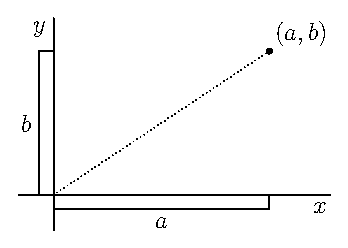
\includegraphics[width=7cm]{figure01.eps}
\caption{Cartesian Coordiantes in $\RR^2$}
\label{Cartesian Coordiantes}
\end{figure}
\clearpage

The basic idea of cartesian coordinates should be familiar to
you from high school level mathematics. In the plane, 
cartesian coordinates are formed by choosing
a center point, drawing two perpendicular directions called axes
(usually, but not necessarily, labelled $x$ and $y$), and
describing each point in the plane by two real numbers, written
$(a,b)$, representing how far along each axis the point falls.

We must point out that $a$ and $b$ are always real numbers, at
least by default. Though we frequently deal with integer or
rational coordinates, the system allows for any real numbers to
represent coordinates. Since there are two dimensions in the
plane, we refer to the plane with cartesian coordinates as
$\RR^2$. Similarly, for space with cartesian coordinates
$(a,b,c)$, we write $\RR^3$. The axes in $\RR^3$ are typically called
$x$, $y$ and $z$. 

Though we won't deal with higher dimensions in this course, the
cartesian coordinate system generalizes easily to any number
of dimensions. We can no longer visualize or draw the
geometry in higher dimensions, but we can still work with the
algebraic representation according to the same principles.
For example, in $\RR^5$, there are five axes, all
perpendicular to each other, and points are represented by
five real numbers $(a,b,c,d,e)$, showing the distance along
each of the axes. We write $\RR^n$ for a cartesian system in
general $n$ dimensions. This is one of the most powerful
aspects of cartesian coordinates -- we can now do geometry in
many dimensions and transcend the limitations of our
three-dimensional vision and perception.

\begin{figure}[t]
\centering
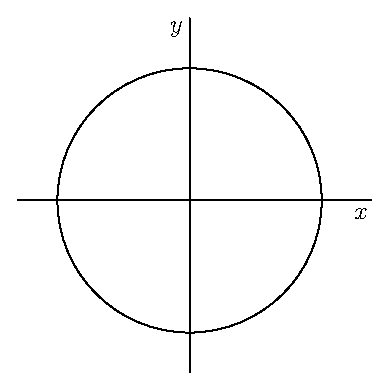
\includegraphics[width=5cm]{figure64.eps}
\caption{The Circle: A Locus}
\label{The Circle}
\end{figure}

Cartesian coordinate are useful for giving
algebraic definitions for various geometric shapes and objects.
For an equation in $x$ and $y$, the coresponding shape consists
of all points $(a,b)$ in the plane which satisfy the equation
when $x$ is replaced by $a$ and $y$ is replaced by $b$. 
Such an collection of points is called \emph{locus} of the
equation. The plural of locus is \emph{loci}.

\begin{figure}[t]
\centering
\begin{subfigure}{.5\textwidth}
 \centering
 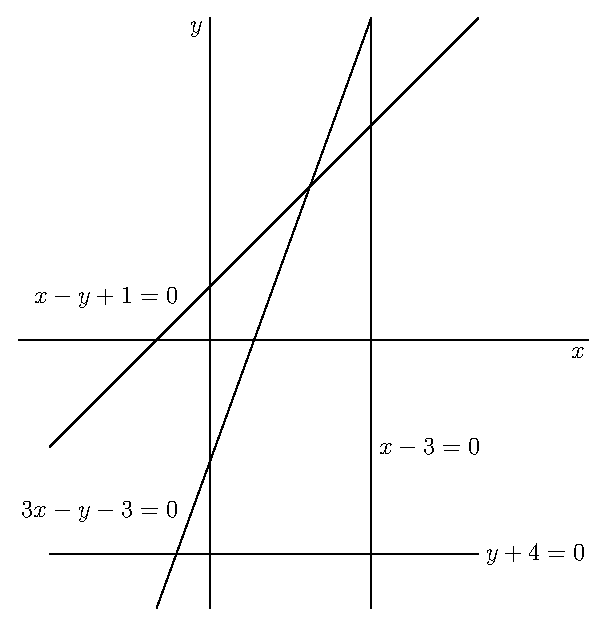
\includegraphics[width=5cm]{figure02.eps}
 \caption{Four Lines}
 \label{Four  Lines}
\end{subfigure}%
\begin{subfigure}{.5\textwidth}
 \centering
 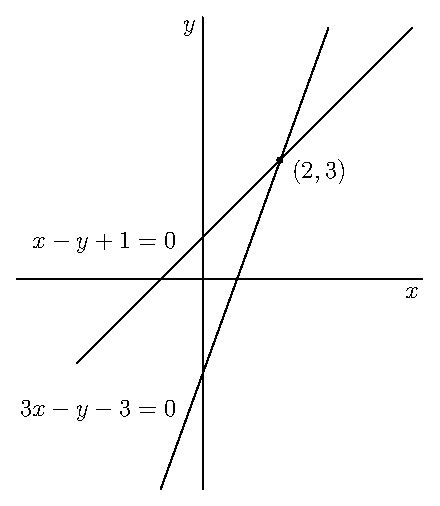
\includegraphics[width=5cm]{figure22.eps}
 \caption{Intersections of Lines}
 \label{Intersections of Lines}
\end{subfigure}
\caption{Lines as Loci}
\label{Lines as Loci}
\end{figure}

The simplest these loci are lines. Lines are given by
equations $ax + by + c = 0$ for constants $a,b,c$. If $b \neq
0$, then this can be converted into the more familiar
slope-intercept form $y = mx + n$ by solving for $y$. Along
with planes and other flat objects, lines are called the
\emph{linear loci}. Linear loci can are loci whose equations
in $x$ and $y$ (or in more variables in higher dimensional
$\RR^n$) involve only degree one polynomials. The subject of
linear algebra is the study of such linear loci and their many
properties.

You will be expected to work with the equations of lines. In
particular, you will need to be able to derive the equation of
the line, both in standard form and slope-intercept form,
given two points or given a point and a slope. This will be
particularly important when we describe tangent lines to
graphs.

You will also be expected to find the intersections of lines.
In Figure \ref{Intersections of Lines}, we have the lines
$y=x+1$ and $y=3-3x$. Finding the intersetion point is
equivalent to finding two coordinates $x$ and $y$ which
satisfy both equations. Algebraically, that is solving the
system composed of both equation.
\begin{align*}
y & = x+1 \\
y & = 3x-3 \\
x+1 & = 3x-3 \\
-2x & = -4 \\
x & = 2 \\
y & = x+1 = 2+1 = 3 \hspace{1cm} \implies \text{The
intersection point is $(2,3)$}
\end{align*}

\chapter{Conics and Loci}
\label{Conics and Loci}

\section*{Conics}

The conics are the second important class of loci. Unlike
the linear loci, these are objects where we allow degree two
polynomials in the coordinate variables. Conics are a very
old topic in mathematics; their names and definitions come
from ancient Greece. They are called conics (short for conic
sections) since they can be formed by taking slices of a
hollow cone at various angles. We will give three equivalent
definitions for each conic: one instrinsically geometric
definition, one as a the slice of a cone, and one by algebraic
equations. For the algebraic equations, we will assume that
the conic is centred at the origin.

\begin{figure}[ht]
\centering
\includegraphics[width=7cm]{figure23.eps}
\caption{Slicing a Cone}
\label{Slicing a Cone}
\end{figure}
\clearpage

\begin{figure}[t]
\centering
\begin{subfigure}{.5\textwidth}
 \centering
 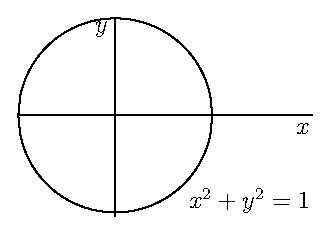
\includegraphics[width=5cm]{figure03.eps}
 \caption{The Circle}
\end{subfigure}%
\begin{subfigure}{.5\textwidth}
 \centering
 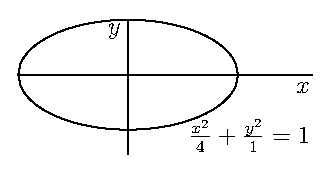
\includegraphics[width=5cm]{figure06.eps}
 \caption{The Ellipse}
\end{subfigure}
\label{Conics 1}
\end{figure}

\begin{description}
\item[The Circle]
\item[Intrinsic Definition] Given a positive real number $r$,
a circle is the set of all points in the plane which are
exactly $r$ units away from the origin. $r$ is called the
radius of the cicle.
\item[Conic Slice Definition] A circle is a perfectly
horizontal slice of a cone.
\item[Algebraic Definition] A circle is described by the
equation $x^2 + y^2 = r^2$.
\end{description}

\begin{description}
\item[The Ellipse]
\item[Intrinsic Definition] Given two points $p$ and $q$ and a
positive real number $r$, the ellipse is the set of all points
in the plane where the sum of the distances to $p$ and $q$ is
exactly $r$. The points are called the foci (singular focus). 
\item[Conic Slice Definition] An ellipse is a slice of a cone
at an angle greater than zero but less than the angle of the
cone.
\item[Algebraic Definition] An ellipse is described by the
equation $\frac{x^2}{a^2} + \frac{y^2}{b^2} = 1$. Assuming
that $a>b$, the foci are at $(\sqrt{a^2-b^2},0)$ and
$(-\sqrt{a^2-b^2},0)$. The length $a$ is called the semi-major
axis and the length $b$ is called the semi-minor axis.
\end{description}

\begin{figure}[b]
\centering
\begin{subfigure}{.5\textwidth}
 \centering
 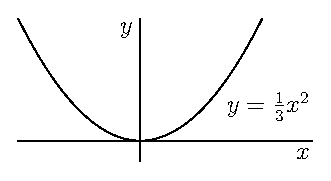
\includegraphics[width=5cm]{figure05.eps}
 \caption{The Parabola}
\end{subfigure}%
\begin{subfigure}{.5\textwidth}
 \centering
 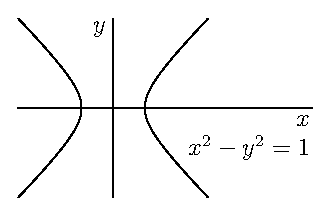
\includegraphics[width=5cm]{figure04.eps}
 \caption{The Hyperbola}
\end{subfigure}
\label{Conics 2}
\end{figure}
\clearpage

\begin{description}
\item[The Parabola]
\item[Intrinsic Definition] Given a positive real number $r$,
a point $p$ and a line $L$, the parabola is the set of all
points in the plane which are equidistant to the point $p$
and the line $L$. The point $p$ is called the focus and the
line $L$ is called the directrix
\item[Conic Slice Definition] A parabola is a slice of the cone
at exactly the angle of the cone.
\item[Algebraic Definition] A parabola is described by the
equation $y = ax^2$. The focus is $(0,\frac{a}{4})$ and the
directrix is $y=\frac{-a}{4}$. 
\end{description}

\begin{description}
\item[The Hyperbola]
\item[Intrinsic Definition] Given two points $p$ and $q$ and a
positive real number $r$, the hyperbola is the set of all points
in the plane where the difference of the distances to $p$ and $q$ is
exactly $r$. The points are called the foci (singular focus). 
\item[Conic Slice Definition] A hyperbola is slice of a cone at
an angle steeper than the angle of the cone.
\item[Algebraic Definition] A hyperbola is described by the
equation $\frac{x^2}{a^2} - \frac{y^2}{b^2} = 1$
\end{description}

One of the major motivating problems for conics and analytic
geometry is the problem of
celestial motion -- how planets, moons, stars, comets and other
celestial objects move and orbit around each other. The Greeks
assumed, erroneously, that orbits ought to be perfect circles.
Johannes Kepler, in the 16th century, correctly observed that
orbit take non-circular shapes. He put forward a very
convincing theory that orbits have shapes which are conics with
the larger object fixed at one of the foci of the conic. This
leads to ellipses for objects without escape velocity and
hyperbolas for those with escape velocity. Though not perfect
(particularly in complicated multi-body problems or when
relativistic corrections are included), Kepler's model is
remarkably accurate. Conics are still used as the basic
models of orbital paths.
\clearpage

\section*{Other Loci}

\begin{figure}[ht]
\centering
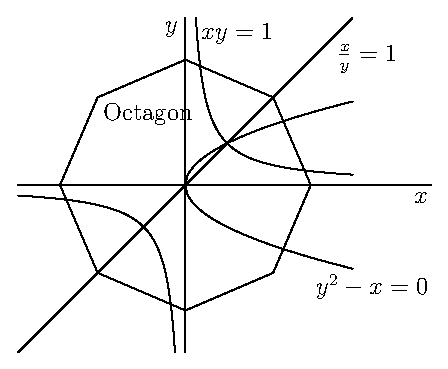
\includegraphics[width=6cm]{figure07.eps}
\caption{Several Other Loci}
\label{Several Other Loci}
\end{figure}

Lines and conics are just two of many classes and families of
loci in $\RR^2$. Here are some others.
\begin{smallitemize}
\item A curve in $\RR^2$: While curves include lines and
conics, the term `curve' is a general term for curving paths.
Many equations give rise to complicated curves, which can 
be very unpredicable. Future calculus courses will study the
calculus of cuves.
\item Instead of lines, we can restrict to portions of lines.
For example, the piece of the line $y=x$ that has only positive
$x$ coordinates is the ray pointing out from the origin at an
angle of $\pi/4$ radians. By taking finite pieces, we get line
segments.
\item With line segments, we can form straight-edged objects
such as polygons. They are also loci not defined by one
particular equation, but by the equations of several lines and
restriction of those lines.
\end{smallitemize}
These are far from the only examples. Curves and loci can be
very complicated: they can double back and self intersect,
they can be jagged and disconnected, and they can even be very
strange fractal-like space filling curves. Consider the locus
of the equation $x^2 + y^2 =0$. Though this is a reasonable
equation in the coordinate variables $x$ and $y$, this locus
only has one point: $(0,0)$. Since $x^2$ and $y^2$ are always
positive, no other values satisfy. Worse, consider $x^2 + y^2
= -1$. This locus has no points at all.

\begin{figure}[t]
\centering
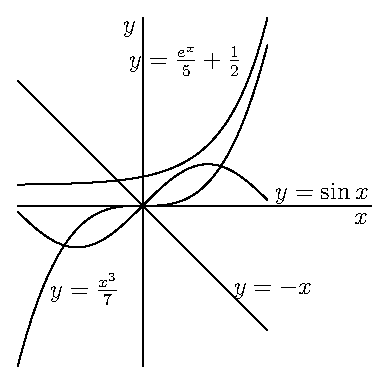
\includegraphics[width=6cm]{figure08.eps}
\caption{Four Graphs}
\label{Four Graphs} 
\end{figure}

Graphs of functions are also loci. If $f(x)$ is a real-valued
function, then the locus $y = f(x)$ is the graph of that
function. Note that the graph itself is not the function, but
just a geometric picture or representation of what the
function does. 

Since each value $x$ leads to at most one function value $f(x)$,
the graph of a function has the important property that for any
fixed value $x$, there is only one point of the locus with that
$x$ coordinate. This is usually refered to a a vertical line
test -- a vertical line can cross the graph of a function at
most once. Many of the loci we've seen above do not satisfy
this; therefore, they cannot be graphs of functions. In
addition, graphs never double back and never self-intersect. 

\begin{figure}[b]
\centering
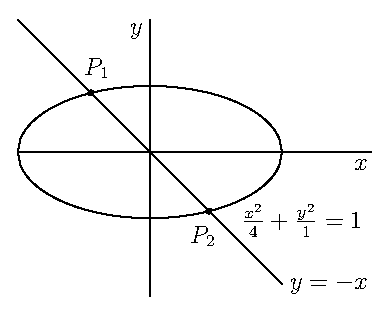
\includegraphics[width=6cm]{figure24.eps}
\caption{Intersection of a Line and an Ellipse}
\label{Intersection of a Line and an Ellipse}
\end{figure}

\section*{Intersection}

Intersection is a key idea in analytic geometry. Given two
loci in $\RR^n$, we often want to know if they intersect.
In diagram \ref{Intersection of a Line and an Ellipse}, the
ellipse $\frac{x^2}{4} + \frac{y^2}{1} = 1 $ and
the line $y=-x$ have two intersection points:
$p_1 = (\frac{-2}{\sqrt{5}},\frac{2}{\sqrt{5}})$ and
$p_2 = (\frac{2}{\sqrt{5}},\frac{-2}{\sqrt{5}})$ 

As with intersection of lines, finding the intersection of
loci is the same as asking for common solutions of the 
equations. Solving systems of equations is one of the most
basic tasks in mathematics. and intersection is the geometric
interpretation.

\section*{Shifts}

\begin{figure}[t]
\centering
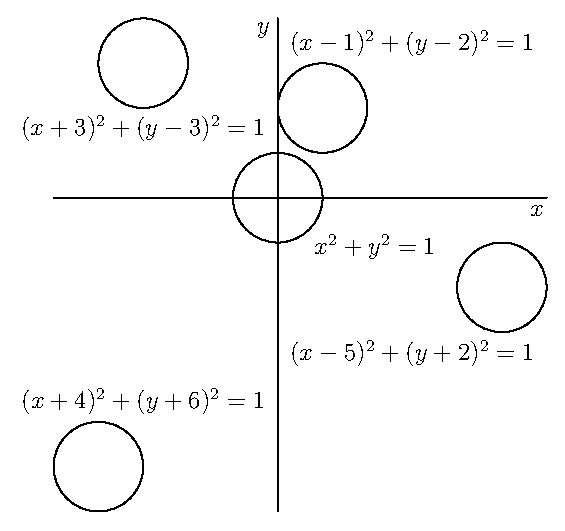
\includegraphics[width=7cm]{figure25.eps}
\caption{Shifts of a Circle}
\label{Shifts of a Circle}
\end{figure}

For conics, I noted that all of the conic equations were
centered at the origin. By understanding shifts of loci, we
learn how to write conics centered at any point. Shifts are a
process of changing the equation of a locus to move the locus
around the plane. 

Let $a$ be a positive real number and consider the equation of
a locus.
\begin{smallitemize}
\item If we replace all instance of $x$ by $x-a$, we move the
locus $a$ units in the positive $x$ direction.
\item If we replace all instance of $x$ by $x+a$, we move the
locus $a$ units in the negative $x$ direction.
\item If we replace all instance of $y$ by $y-a$, we move the
locus $a$ units in the positive $y$ direction.
\item If we replace all instance of $y$ by $y+a$, we move the
locus $a$ units in the negative $y$ direction.
\end{smallitemize}
Consider the cirlce $x^2 + y^2 = 1$, which is a circle of
radius one centered at the origin. Figure \ref{Shifts of a
Circle} shows the following shifts.
\begin{smallitemize}
\item The locus $(x-1)^2 + (y-2)^2 = 1$ is a circle of radius
1 centered at $(1,2)$.
\item The locus $(x+3)^2 + (y-3)^2 = 1$ is a circle of radius
1 centered at $(-3,3)$.
\item The locus $(x+4)^2 + (y+6)^2 = 1$ is a circle of radius
1 centered at $(-4,-6)$.
\item The locus $(x-5)^2 + (y+2)^2 = 1$ is a circle of radius
1 centered at $(5,-2)$.
\end{smallitemize}
Shifts do not only apply to conics: we can shift any locus in
this way.

\chapter{Functions}
\label{Functions}

\section*{Definitions}

In order to define functions, we need to define sets. A
\emph{set} is any collection of things; the things in a set
are called its \emph{elements} While most of our sets will be
sets of numbers, apriori a set can have any kind of elements. 
Particularly useful sets for this course are the standard
number sets ($\NN$, the natural numbers; $\ZZ$, the integers;
$\QQ$, the rational number, $\RR$, the real numbers), open
inverals $(a,b)$ and closed interval $[a,b]$.

Let $A$ and $B$ be sets. 
A \emph{function} $f: A \rightarrow B$ is a rule that assigns an
element of $B$ to each element of $A$. The set $A$ is called
the domain. The range of the function is the subset of $B$
consisting of all outputs of the function.

There are three major interpretations of functions.
First, we can think of a function as a machine which acts on
things. The function $f(x) = x^2$ from $\RR \rightarrow
\RR$ is a rule which assignes to each number its square.
However, it's often more natural to think of $f$ as the thing that
squares numbers. Functions are agents which
perform actions. 

Second, we think of functions as relationships and
dependencies. When we have a function $f: A \rightarrow B$,
we can thing of the elements of $B$ depending on the elements
of $A$. If we say that population growth is a function of
food supply, we mean that there is a function which goes from
numbers representing food suply to numbers representing growth
rates. That function encodes the dependance of growth on food
supply.

Lastly, we often visualize a function by its graph. See the
library of functions reference sheet for graphs of many common
functions. Visualizing the action of a function by its graph is
a very convenient way to remember the function and its
properties.

\section*{Functions on $\RR$}

For the purposes of calculus, we will deal with functions
defined on $\RR$ and its subsets. For most functions, we will
not explicitly stipulate a domain; the domain of the function
will implicitly be the largest subset of real numbers where
the function applies. Likewise the range will be the subset
of all possible outputs of the function.

Determining the domain of a function on $\RR$ means avoiding
illegal mathematical actions. There are three common restrictions.
\begin{smallitemize}
\item We cannot divide by zero.
\item We cannot take even roots of negative numbers.
\item We cannot take logarithms of negative numbers or zero.
\end{smallitemize}
There are special domain restrictions for certain
functions, such as inverse trig functions, but the main three
cover the vast majority of functions we will be dealing with.
Determining the domain of a function $f$ means excluding real
numbers which would lead to one of the three problems.

In addition, should we wish to, we can put additional domain
restrictions on a function. Functions of time cannot extend
infinitely back in time, so we usually stipulate a starting
time; the domain of the function will be after that starting
time. Restricting domains is also useful to make a function
invertible.

\section*{Types of Functions}

We want to give a catalog of the common types of functions we
encounter in calculus.

\subsection*{Constant Functions}

\begin{figure}[t]
\centering
\begin{subfigure}{.5\textwidth}
 \centering
 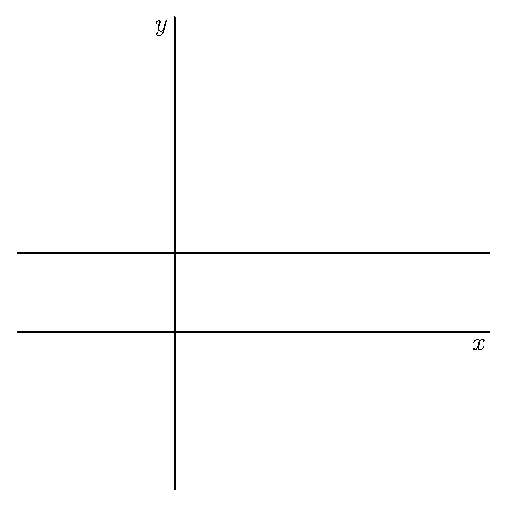
\includegraphics[width=5cm]{figure26.eps}
 \caption{A Constant Function}
\end{subfigure}%
\begin{subfigure}{.5\textwidth}
 \centering
 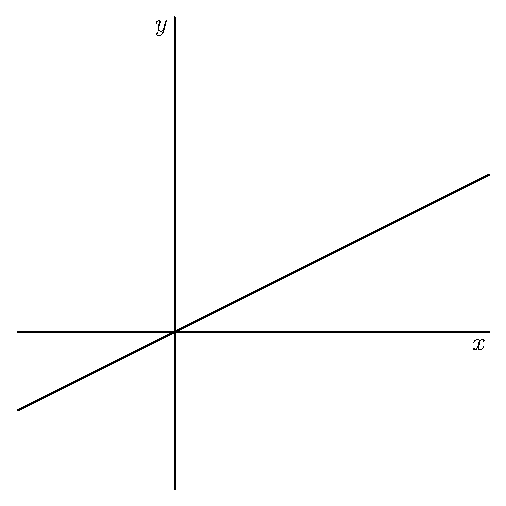
\includegraphics[width=5cm]{figure27.eps}
 \caption{A Linear Function}
\end{subfigure}
\label{Types of Functions 1}
\end{figure}

The simpliest kind of function is a constant function. Its
output is the same regardless of input. The function
$f(x) = 5$ is constant at 5: it will give the value 5 no
matter what value of $x$ we specify. Constant functions have
no domain restrictions.

\subsection*{Linear Functions}

Linear functions have the form $f(x) = ax + b$ for real
numbers $a$ and $b$. Their graphs which are straight lines,
hence the name `linear'. Linear functions includes constant
functions, since we allow $a=0$. All the tools from analytic
geometry for understanding lines are useful for understanding
linear functions. Linear functions have no domain
restrictions. 

A particularly important linear function is the function $f(x)
= x$, which is called the \emph{Identity Function}. It is the
unique function which takes any input and gives that input back
without any action.

\subsection*{Quadratic Functions}

Quadratic functions have the form $f(x) = ax^2 + bx + c$.
Their graphs are parabolas. We have a large array of
tools to understand parabolas, including the vertex-form (to find
the highest/lowest point of the function) and the quadratic
equation (to find the roots). Quadratic functions have no
domain restrictions.

\vspace{1cm}

\begin{figure}[ht]
\centering
\begin{subfigure}{.5\textwidth}
 \centering
 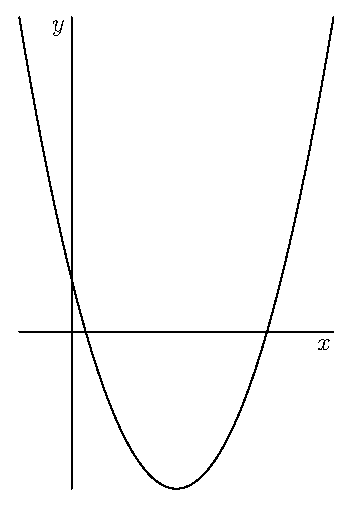
\includegraphics[width=4cm]{figure33.eps}
 \caption{A Quadratic Function}
\end{subfigure}%
\begin{subfigure}{.5\textwidth}
 \centering
 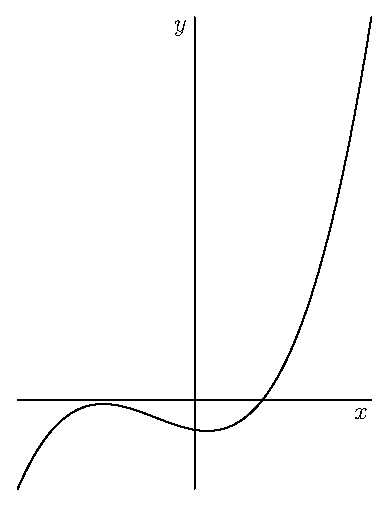
\includegraphics[width=4cm]{figure28.eps}
 \caption{A Polynomial Function}
\end{subfigure}
\label{Types of Functions 2}
\end{figure}

\subsection*{Polynomial Functions}

Polynomial functions have the following form, where the $a_i$
are anyreal numbers.
\begin{equation*}
f(x) = a_nx^n + a_{n-1}x^{n-1} + \ldots + a_2x^2 + a_1 x + a_0
\end{equation*}
The number $n$ of the largest power in the polynomial is
called the \emph{degree} of the polynomial. The previous
cases are all polynomials: constant functions have degree
zero, linear functions have degree one, and quadratics have
degree two. We have names for the next few degress as well:
cubics have degree three, quartics have degree four and
quintics have degree five. Polynomial functions have a
familiar standard shape involving a graph that curves up a
down some number of times. The maximum number of times the
graph of polynomial can change directions is one less than the
degree. Polynomials of degree $n$ can have at most $n$ roots,
though they may have fewer. Polynomial functions have no
domain restrictions. 

\subsection*{Rational Functions}

Rational numbers are fractions involving integers, In the same
way, rational functions are fractions involving polynomials.
Rational functions have the follwoing form, where $p(x)$ and
$q(x)$ are polynomials.
\begin{equation*}
f(x) = \frac{p(x)}{q(x)} 
\end{equation*}
Rational functions may have domain
restrictions. Into order to avoid dividing by zero, we must
avoid $x$ where $q(x) = 0$. Rational functions may have
\emph{vertical asymptotes} near their underfined points. A
vertical asymptote is a vertical line which the graph of the 
function approaches near an undefined point. 

\begin{figure}[b]
\centering
\begin{subfigure}{.5\textwidth}
 \centering
 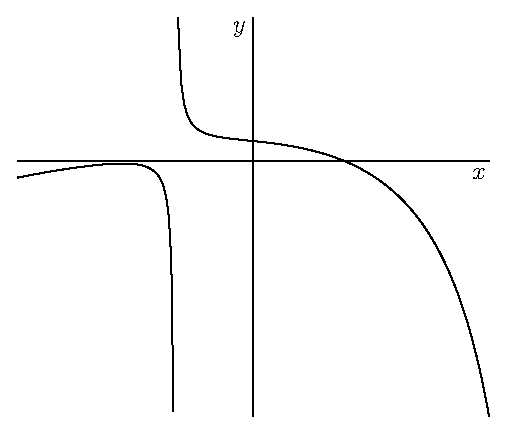
\includegraphics[width=5cm]{figure29.eps}
 \caption{A Rational Function}
\end{subfigure}%
\begin{subfigure}{.5\textwidth}
 \centering
 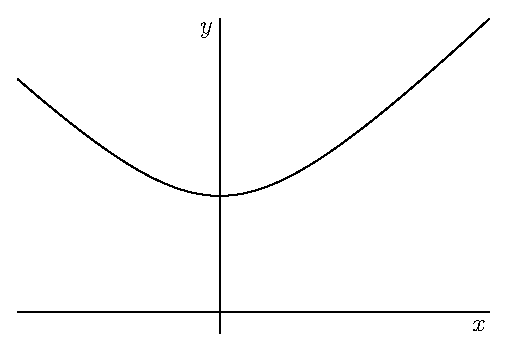
\includegraphics[width=5cm]{figure30.eps}
 \caption{An Algebraic Function}
\end{subfigure}
\label{Types of Functions 3}
\end{figure}

\subsection*{Algebraic Functions} 

We are now moving into much broader categories of functions,
where it is impossible to give a cohesive sense of the
behaviour of the functions. Terminology is still useful for
grouping these functions. Algebraic functions are
functions which involve the four basic operations of addition,
subtraction, multiplication and division as well as any real
exponent. This includes polynomials and rational functions,
but also roots, since roots can be written as fractional
exponents. ($\sqrt{x} = x^{\frac{1}{2}}$). Algebraic
functions can be very complicated conglomerations of these
operations. 

\subsection*{Trigonometric Functions}

\begin{figure}[b]
\centering
\begin{subfigure}{.5\textwidth}
 \centering
 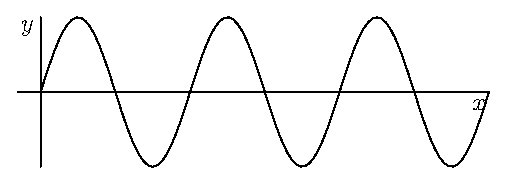
\includegraphics[width=6cm]{figure32.eps}
 \caption{A Trigonometric Function}
\end{subfigure}%
\begin{subfigure}{.5\textwidth}
 \centering
 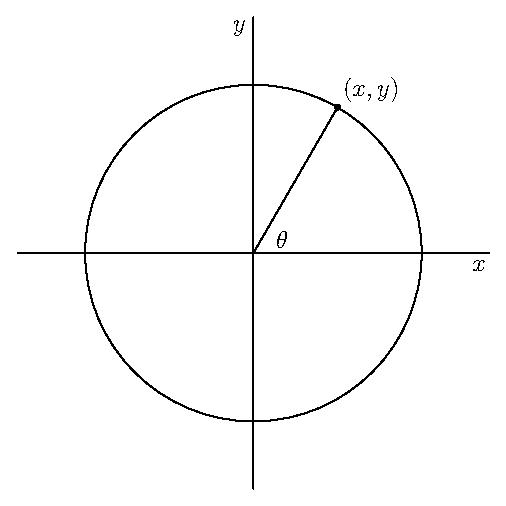
\includegraphics[width=5cm]{figure34.eps}
 \caption{Trigonometry and the Circle}
\end{subfigure}
\label{Trigonometric Functions}
\end{figure}

The first type of non-algebraic functions are trigonometric
functions.  Sine and cosine have the familiar sinusoidal wave
shape: infinitenly many oscilation which repeat perfectly
with some period. Sine and cosine waves can be analyzed by
their amplitude and period. The other trigonometric functions
(tangent, cotangent, secant and cosecant) are also periodic,
but they have undefined points and vertical asymptotes at
regular intervals. 

Though the trigonometric functions are usually associated to triangles,
it is more natural to define them using the circle. If
$\theta$ is the angle from the positive $x$ axis, then $\cos
\theta$ is exactly the $x$ coordinate of the circle and $\sin
\theta$ is exactly the $y$ coordinate of the circle. All of
the important properties of trigonometric functions can be
derived from circle geometry, including the many trigonometric
identities. Please see the formlua reference sheet for
definitions and identities involving trigonometric functions.

Each trigonometric function has a inverse function. There are
two standard notations; the inverse of $\sin(x)$ is written
either as $\sin^{-1}(x)$ or $\arcsin(x)$. Even though the
former notation is familiar from calculators, we will use the
latter in these notes to avoid confusions with
$\frac{1}{\sin(x)}$.

\subsection*{Exponential and Logarithmic Functions}

\begin{figure}[t]
\centering
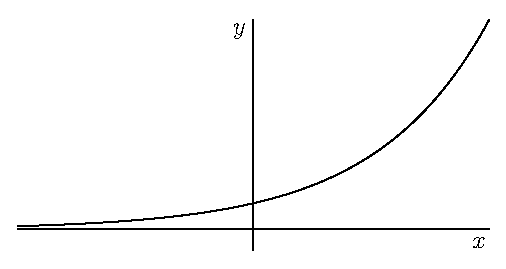
\includegraphics[width=8cm]{figure31.eps}
\caption{An Exponential Function}
\label{An Exponential Function}
\end{figure}

If $a$ is a positive real number, then functions of the form
$f(x) = a^x$ are called exponential functions. They differ
from roots and polynomials in that the variable is in the
exponent. This distinction is very important but easy to
confuse: $f(x) = x^a$ is an algebraic function but $f(x) =
a^x$ is an exponential function, which is not algebraic.
The laws of exponents (see the formula sheets) help us work
with exponential functions.

The exponential bases you've most likely seen to
date have been 2 and 10. These are useful bases, but in
calculus (for reasons that will become clear later) we prefer
a different base. The irrational number $e$ is called Euler's
number. It has an approximate
value $e = 2.71828\ldots$. It is by far the most common
exponential base; you will be seeing the exponential function
$f(x) = e^x$ very frequently. It is reasonable to claim that 
$f(x) = e^x$ is the most important function in calculus.

The inverse of the exponential function is the logarithm. If the
exponential has base $a$, its logarithm is written
$\log_a x$. However, the inverse of the exponential $f(x) =
e^x$ is instead written $\ln x$ and
called the natural logarithm. We
will almost exclusively deal with the natural logarithm in
calculus. Logarithms (in any base) can only act on positive
numbers.

\subsection*{Hyperbolic Functions}

Though we won't define or investigate these function until
Calculus II, it is useful to mention that there is a third important
family of non-algebraic functions called the hyperbolics
functions. There are a strange family, in some ways similar
to trigonometric functions and in some ways similar to
exponentials. They have inverse functions as well, called the
inverse hyperbolics. 

\subsection*{Elementary Functions}

\begin{figure}[t]
\centering
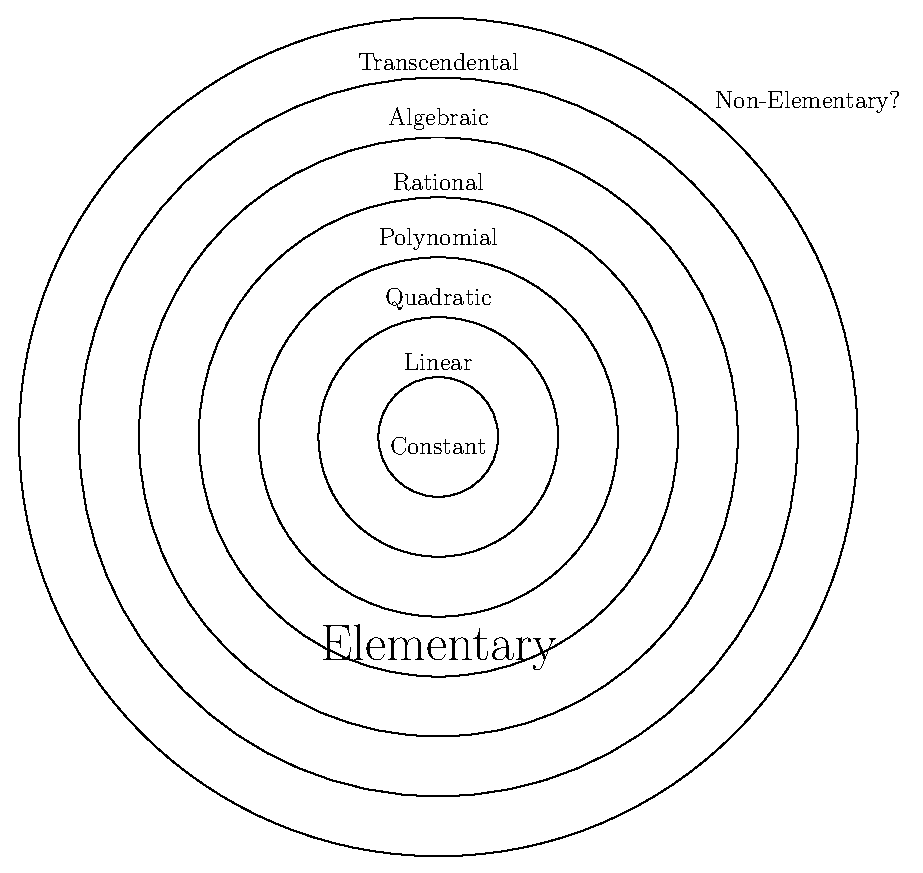
\includegraphics[width=12cm]{figure35.eps}
\caption{The Universe of Functions}
\label{The Universe of Functions}
\end{figure}

Everything we've defined so far comes together to form the
large family refered to as the elementary functions. We can think
of elementary functions as those function for which we have a
familiar and succinct notation. Everything we've defined so far,
as well as any combination of these functions, is an
elementary function. As we will see later, calculus gives us
methods for defining many non-elementary functions. Depending
on how far you proceed through the calculus stream, you will
see a few or many of these non-elementary functions.
\clearpage

\section*{Properties of Functions}

We use a number of properties of functions to describe their
behaviour.
\begin{smallitemize}
\item The \emph{domain} of a function is all possible real
inputs to the function. The domain can be
restricted to a smaller subset if desired.
\item The \emph{range} of a function is all possible real
outputs of the function.
\item A function is \emph{even} if $f(-x) = f(x)$. Visually,
the graph of the function has a mirror-image symmetry over the
$y$ axis.
\item A function is \emph{odd} if $f(-x) = -f(x)$. Visually,
the graph of the function is the preserved under a half-turn
rotation about the origin.
\item A function is \emph{periodic} if there is a real number
$a$ such that $f(x+a) = f(a)$ for all $x$. The smallest positive
real number $a$ that satisfies is called the period.
\item A function is called \emph{increasing} if $a<b$ implies $f(a) <
f(b)$. Visually, the graph of the function is growing upwards
as the input increases. 
\item A function is called \emph{decreasing} if $a<b$ implies
$f(a) > f(b)$. Visually, the graph of the function is
declining downwards as the input increases.
\item A function is called \emph{monotonic} if it is either
always increasing or always decreasing. 
\item A function is \emph{bounded above} if there is a number $A$
such that $f(x) < A$ for all $x$. Visually, the graph of the
function never gets above the height $y=A$.
\item A function is \emph{bounded below} if there is a number $B$
such that $f(x) > B$ for all $x$. Visually, the graph of the
function never gets below the height $y=B$.
\item A function is \emph{bounded} if it is both bounded above and
below. That is, there exists numbers $A$ and $B$ such that $B
< f(x) < A$ for all $x$. Visually, the function remains
within the range $y \in [A,B]$ for any input.
\item A \emph{$y$-intercept} of a function is a place where it
crosses the $y$ axis. Since a function satisfies a vertical
line test, there is only one possible $y$ intercept found at
$f(0)$ (if $0$ is in the domain).
\item An \emph{$x$-interceopt} or \emph{root} of a function is
a place where it crosses the $x$ axis or, equivalently, has
the output $f(x) = 0$. 
\end{smallitemize}

\chapter{Operations on Functions}
\label{Operations on Functions}

\section*{Pointwise Operations}

The most familiar way to put functions together is through the
conventional operations of arithmetic: addition, subtraction,
multiplication, division and exponentiation. If $f$ and $g$
are functions, then $f+g$, $f-g$, $f \cdot g$, $\frac{f}{g}$
and $f^g$ are all functions. They may have additional domain
restrictions, such as avoiding the roots of $g$ in
$\frac{f}{g}$. We call these combinations \emph{pointwise
operations} on function. 

\section*{Composition}

A more novel way to combine function is \emph{composition}.
In pointwise operations, both the functions act seperately on
the input and then we combine the result. In composition, we
let one function act first and then let the second act on the
output of the first. If $f$ and $g$ are functions, we write
$f \circ g$ or $f(g(x))$ for their composition. In this
notation, somewhat counterintuitively, the function on the
right acts first. $f \circ g$ means we let the function $g$
act first and then let the function $f$ act second. Additional
domain restrictions may result from composition, since the
output of $g$ must be acceptable input for the function $f$.
In $f \circ g$, we call $g$ the \emph{inside function} and $f$
the \emph{outside function}.

\begin{example}
If $f(x) = e^x$ and $g(x) = x^2+1$, then
$f \circ g (x) = e^{x^2+1}$ and $g \circ f = (e^x)^2
+1$. 
\end{example}

\begin{example}
Often is it important to recognize a composed functions and
identify the pieces of the composition. 
The function $h(x) = \sqrt{x+7}$ is a composition with inside
function $g(x) = x+7$ and outside function $f(x) = \sqrt{x}$.
For complicated functions, there may be several ways to
decompose the function as a composition; finding various
decompositions and knowing which composition to use is an
important skill.
\end{example}

Composition can be iterated. If $f$, $g$ and $h$ are
functions, $f \circ g \circ h(x)$ is the composition of all
three, with $h$ acting first, $g$ second and $f$ third. 

\section*{Inversion}

The last important operation on functions is inversion.
Inversion attempts to undo what a function has accomplished,
to go backwards and return the output to the original input.
If $f(x)$ is a function, we write $f^{-1}(x)$ for its inverse.
This notation \emph{does not} mean the reciprocal function
$\frac{1}{f(x)}$. 

In order for a function to be invertible, each output needs to
go back to a unique input. This restrictions implies that  no
two inputs can be sent to the same output. This property is
called \emph{injectivity}, but for our purposes, it is enough
that a function is \emph{monotonic}. A function which always
increases or decreases can only have one input sent to any
particular output; therefore, it is invertible.  When we want
to invert a function, we must make sure that it is monotonic.

When we compose a function and its inverse, we get the
original input back. That is $f \circ f^{-1}(x) = x$ and
$f^{-1} \circ f(x) = x$ on the approriate domains. This is
very useful for manipulating equations, since we can remove
any function by compositing with its inverse. 

\begin{example}
We use the natural logarithm to remove the exponential with
base $e$.
\begin{align*}
e^x & = y \\
\ln e^x & = \ln y \\
x & = \ln y
\end{align*}
\end{example}

\begin{example}
Likewise, we use inverse trig to remove trig function.
\begin{align*}
\sin x & = y \\
\arcsin (\sin x) &= \arcsin y \\
x & = \arcsin y
\end{align*}
\end{example}

For a monotonic function, the domain of the inverse will be
the range of the original function. If we can calculate the
range of the original function, we get the domain of the
inverse for free. In the first example above, the range of
$e^x$ is $(0,\infty)$, so that becomes the domain of $\ln x$.
In the second second above, $\sin x$ is not monotonic on its
whole domain, so we have to make an adjustment before we can
understand the range. 
\clearpage

\section*{Restriction of Domain}

\begin{figure}[t]
\centering
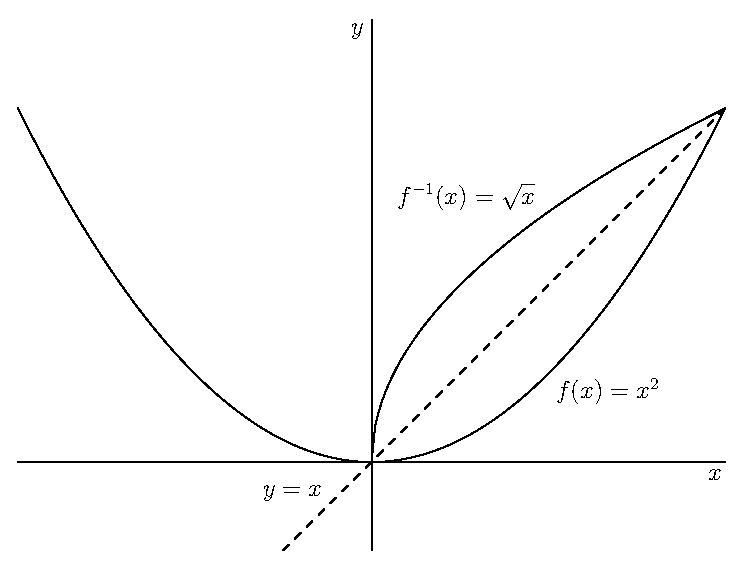
\includegraphics[width=10cm]{figure36.eps}
\caption{Restricting the Domain of $f(x) = x^2$}
\label{Restriction of Domain}
\end{figure}

Many functions are not monotonic, but we would like to invert
them anyway. We solve this problem by restricting the domain.
The classic example is the quadratic $f(x) = x^2$. This
function has a domain of $\RR$, but it is not invertible,
since both $x$ and $-x$ are sent to $x^2$. Going backwards,
we do not know whether to sent $x^2$ to $x$ or $-x$.
Therefore, we restrict the domain. The function $f(x) = x^2$
on the restricted domain $[0, \infty)$ is increasing,
therefore it is invertible. Its inverse is $f^{-1}(x) =
\sqrt{x}$, returning the positive square root.

The example of $\sin x$ we used above is desperately not
monotonic: it isolates up and down constantly. We have to make
a severe restriction to invert it, by choosing a very small
piece where it is monotonic. For $\sin x$, the conventional
choice is the interval $\left[ \frac{-\pi}{2}, \frac{\pi}{2}
\right]$, where $\sin x$ is an increasing function. On this
interval, the range of $\sin x$ is $[-1,1]$, so the domain of
$\arcsin x$ is also $[-1,1]$. 

\chapter{Models}
\label{Models}

In this course, we use the term `model' in the broadest
possible mathematical sense: a model is any application of a
mathematical concept to an external situation.  Since calculus
is the study of functions, our models will be functions chosen
to describe an observed connection between two quantities. The
branch of mathematics that deals with models is called applied
mathematics.

Models are the mathematical versions of the scientific method.
If we observe a relationship between two quantities, choosing
a function to describe that relationship is a scientific
hypothesis. We can then work with the mathematics to
understand the function. The behaviour of the function can be
then tested against data, either the original data or new
data. We can re-evaluate to see if the model fits the data to
an acceptable precision.

Our analysis of functions helps us understand models. 
We can ask questions about functions inspired by
their applied context. We'll  start with three important
questions.

\begin{smallitemize}
\item Do we restrict the domain to make it reasonable? A
mathematical model where the independant variable is human
population would reasonably impose restriction that the
population must be positive and bounded above by some maximum
population. These restrictions of the model exist in addition
to whatever natural mathematical restrictions we already have
on domain.
\item We can ask abour starting values. If our model depends
on time, we can set a starting time (often but not necessarily
$t=0$) and specify a value for the function at the starting
time. Even though there is a mathematical description of what
happens before the starting time, we can ignore it since it
doesn't apply to the situation we are modelling.
\item We can ask about the constants in our model. Functions
often involve constants apart from the variables, such at the
coefficients of a polynomial. In a model, the constants should
have reasonable meaning and interpretation. 
\end{smallitemize}

The analysis of models thus consists of everything we used to
analyze functions in Sections \ref{Functions} and
\ref{Operations on Functions} as well as these new
questions. Often we will want a qualitative analysis of the
model. Understanding the general shape and behaviour of the
functions involved is invaluable to this qualitative analysis.
A major goal for this course is to develop tools and
competencies to allow students to analyze functions and
models both quantitatively and qualitatively. The
qualitative analysis can often be expressed in a narrative:
what story is the function telling about the relationship? If
the independant variable is time, as it often is, what is the
story of the dependant variable over a time span? What
happens to it? 

\section*{Regression}

One of the greatest challenges of applied mathematics is
choosing appropriate models. If the real world provides us
with a set of data points, how do we choose a function?
Often we can intuit what kind of function (linear, polynomial,
exponential, etc) we think might fit the data. However, it is
very difficult to be more specific just through intuition.
Once we've chosen a type of function for our model,
\emph{regression} is a set of techniques that help to find the
best specific function for the data.  In this course, we will
only be looking at regressions graphically. The hard work of
calculating functions in a regression is left for future
courses. 

\begin{figure}[ht]
\centering
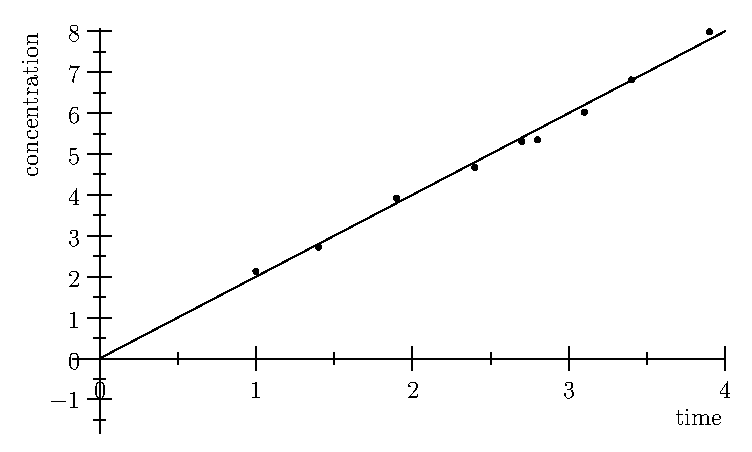
\includegraphics[width=12cm]{figure37.eps}
\caption{A Linear Regression}
\label{A Linear Regression}
\end{figure}

\begin{figure}[ht]
\centering
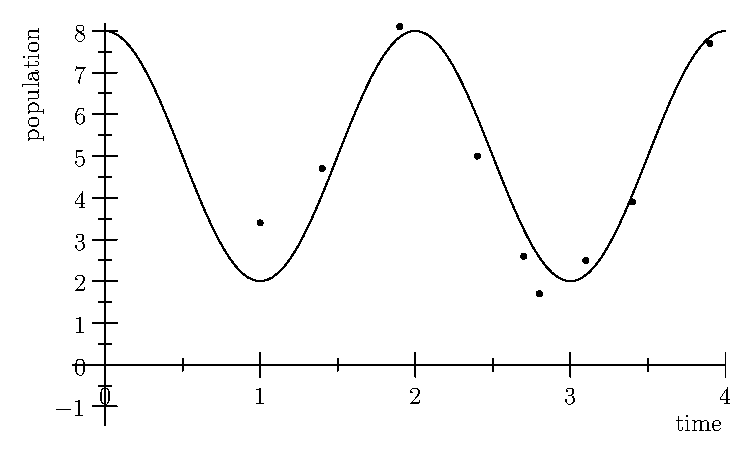
\includegraphics[width=12cm]{figure38.eps}
\caption{A Sinusoidal Regression}
\label{A Sinusoidal Regression}
\end{figure}

\begin{figure}[ht]
\centering
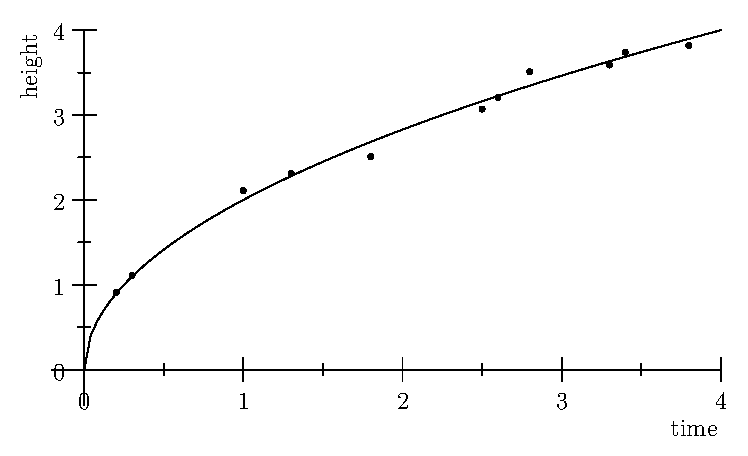
\includegraphics[width=12cm]{figure39.eps}
\caption{A Square-Root Regression}
\label{A Square-Root Regression}
\end{figure}

\chapter{Population Growth}
\label{Population Growth}

A very natural motivating problem is population growth.
Here are some reasonable mathematical questions we might ask
about population.
\begin{smallitemize}
\item How do we encode population growth as a function?
\item What factors affect the growth of population?
\item What is the long-term behaviour of a population?
\item What is the growth rate of a population?
\end{smallitemize}
To encode population growth as a function, we chose a  
function $p(t)$ representing population ($p$) in terms of the
independant variable time ($t$). 

\begin{figure}[hb]
\centering
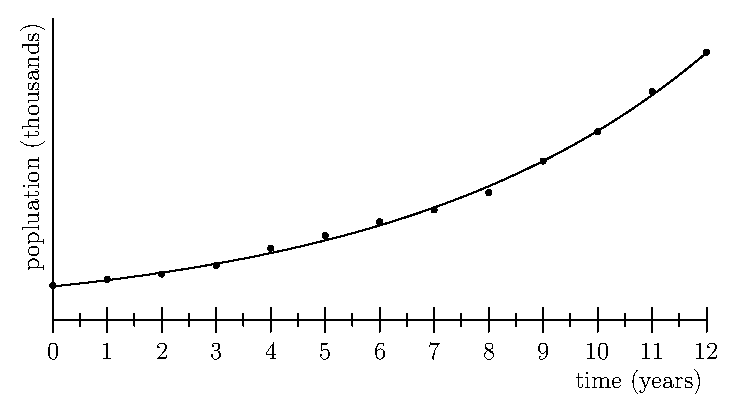
\includegraphics[width=10cm]{figure40.eps}
\caption{An Exponential Regression}
\label{An Exponential Regression}
\end{figure}

\begin{table}[h]
\begin{tabular}{lll}
Year & Population & Growth Rate
\vspace{.3cm} \\
0 & 1032 & Not Applicable \\
1 & 1214 & 17.6 \% \\
2 & 1372 & 13.0 \% \\
3 & 1629 & 18.7 \% \\
4 & 2143 & 31.6 \% \\
5 & 2520 & 17.6 \% \\
6 & 2940 & 16.7 \% \\
7 & 3292 & 12.0 \% \\
8 & 3813 & 15.8 \% \\
9 & 4757 & 24.8 \% \\
10 & 5632 & 18.4 \% \\
11 & 6842 & 21.5 \% \\
12 & 8010 & 17.1 \% 
\end{tabular}
\end{table}

Consider this data set for a population (where $t$ is
counted in years). This growth looks exponential. We could
apply exponential regression to find an exponential function,
as in Figure \ref{An Exponential Regression}.  However, there
is another way of finding a function to fit this model, using
the growth rates to find a function to fit the data. Algebraic
techniques have a hard time understanding growth rates, or
rates of change in general. In calculus, we will develop a
tool called the \emph{derivative} of a function which will
measure its rate of change. For now, we are going to avoid the
technical definition but work with the idea. We need some
notation. For a function $p(t)$, there are two common ways of
writing the derivative.
\begin{equation*}
p^\prime(t) \hspace{1cm} \frac{dp}{dt}
\end{equation*}
The first notation is called Newton's notation, and the second
is called Leibniz's notation. We will use both in this course
but we will rely on Leibniz's notation most of the time.

The derivative is the rate of change of the function, so for
this model, $\frac{dp}{dt}$ is the growth rate of the
population. The average annual increase in the data above is
$20\%$ growth. That means that the growth rate (the amount of
population added in a year) is $\frac{20}{100}$ (or
$\frac{1}{5}$) times the
current population. We can express this as an equation.
\begin{equation*}
\frac{dp}{dt} = \frac{1}{5} p(t)
\end{equation*}
This is a mathematical translation of the understanding of
percentage growth. An equation of this form, involving a
function and its derivative, is called a \emph{differential
equation} (DE, in short). Very often in applied mathematics,
it is easier to observe the rate of change of a function than
the function itself. This leads to models expressed as 
differential equations. Many of the most important
mathematical models in history are expressed as differential
equations.

The regression provided the function $p(t) = 2^{\frac{t}{4}}$.
We will see later in the course that the solution to this
differential equation is a very similar function.
\begin{equation*}
p(t) = e^{\frac{1}{5} t}
\end{equation*}
Solving differential equations is one of the major goals of
calculus. The solution to this equation leads to the profound
connection between percentage growth rate and exponential
growth: if we observe a percentage growth rate, then the
quantities we are observe should be described by an
exponential function. This is how we know that many
populations grow exponentially, as do functions involving
resource use, radioactive decay, heat dissipation, debt
repayment and investment interest. The importance of the
exponential function is strongly related to its use as the
solution to problems of percentage growth.

DEs gives us a different approach to fiting a function to
data. Instead of just using intuition to choose a class of
functions and regression to get the specific function, we can
look at the growth rates of the function in the data. If we
can make a consistent observation about the growth rates, such
as the observation that they grow by a consistent percentage,
we can write that observation as a differential equation. We
can then (hopefully) solve the differential equation to find
the appropriate function.

Before we worry about solving DEs, we simply want to understand
what they say. Our goals is essentially translation: a
differential equation is a mathematical translation of a
statement about the growth rate of a quantity. We want to be
able to pass both ways between the equation and the associated
statement. We have seen how percentage growth with percentage
$c\%$ translates into an equation.
\begin{equation*}
\frac{dp}{dt} = \frac{c}{100} p
\end{equation*}
We can translate other statements as well. Percentage decay
says that we loose a percentage $c\%$ of the quantity per unit
time. 
\begin{equation*}
\frac{dp}{dt} = -\frac{c}{100} p
\end{equation*}
Not all differential equations are percentage growth. Perhaps
the rate of change is proportional to the square of the
current value. 
\begin{equation*}
\frac{dp}{dt} = c(p(t))^2
\end{equation*}

\chapter{Autonomous Differential Equations}
\label{Autonomous Differential Equations}

\section*{Phase Line Analysis}

At this point in the course, we lack the tools to solve 
differential equations. Instead, we want to do some
qualitative analysis of the differential equation. We will
restrict this analysis to a particular type. A differential
equation where the left-side is just $\frac{dp}{dt}$ and
the right-side is some algebraic expression in $p$ is
called an \emph{autonomous differential equation}. Many
natural models are described by autonomous equations,
including  population growth. There is a lovely
piece of analysis for autonomous equations called the
\emph{phase line analysis}. 

Phase line analysis looks at the right side of the
equation and asks for values of the function $p$ which set the
right side to zero. What does this mean? When
the right side of our differential equation is zero, so the left
side is zero as well. The left side is the growth rate, so that
means the growth rate is (momentarily) zero. These are values 
of the population $p$ where there is no growth. We call these
values \emph{steady states} of the population. If the
population is exactly at its steady state, it will not change;
steady states are constant popluations which do no grow or
decline. For population models, we can make the reasonable
assumptions that $p \geq 0$ and $p=0$ is always a steady
state.

Once we have the steady states, we ask what happens between
each steady state. Assuming that the DE is reasonable, then
between the steady states, the right side will be either
positive or negative. When it is positive, we have a positive
growth rate and the population increases.  When it is
negative, we have a negative growth rate and the population
decreases. This direction of growth, negative or positive, is
called the \emph{trajectory} of the popluation between the
steady states.
\clearpage

Amazingly, this gives us an impressively complete
understanding of the population.
\begin{smallitemize}
\item If the popluation is at a steady state, it doesn't
change.
\item If the popluation is not at a steady state, we look at
the trajectory.
\item If the trajectory is positive, the popluation grows
to the closest larger steady state or infinity.
\item If the trajectory is neagative, the population declines
to the closest smaller steady state or zero.
\end{smallitemize}
We summarize this information is a phase line diagram. We
take a ray representing $p \geq 0$ and put dots on the ray for
the steady states. In between, we put arrows to show the
trajectories. Its best to see the phase line diagrams through
examples.

\begin{example}
\begin{equation*}
\frac{dp}{dx} = p^2 - p
\end{equation*}
The right side is zero when $p=0$ or $p=1$, so those are the
steady states. When $p \in (0,1)$ the derivative is negative,
so the trajectory is decreasing. When $p \in (1, \infty)$, the
derivative is positive, so the trajectory is increasing. This
phase line encodes this information.
\end{example}

\begin{figure}[ht]
\centering
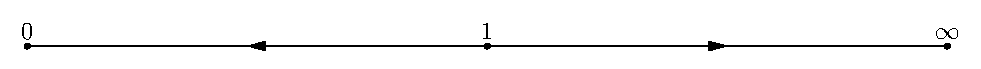
\includegraphics[width=12cm]{figure41.eps}
\caption{The Phase Line Diagram for $\frac{dp}{dx} = p^2 - p$}
\label{Phase Line 1}
\end{figure}

\begin{example}
This is an example of the logistic equation.
\begin{equation*}
\frac{dp}{dt} = 4p-p^2
\end{equation*}
The right side is zero when $p=0$ or $p=4$, so those are the
steady states. When $p \in (0,4)$ the derivative is positive,
so the trajectory is increasing. When $p \in (4, \infty)$, the
derivative is negative, so the trajectory is decreasing. 
\end{example}

\begin{figure}[ht]
\centering
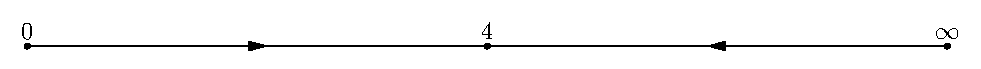
\includegraphics[width=12cm]{figure43.eps}
\caption{The Phase Line Diagram for $\frac{dp}{dt} - 4p - p^2$}
\label{Phase Line 2}
\end{figure}

The logistic equation leads to logistic growth. We can see
from the Figure \ref{Phase Line 2} that the trajectories
all point towards the steady state $p=4$. In logistic growth,
the population wants to approach to some non-zero steady
state. From below, this is growth up to some maximum and from
above it is decay down to a minimum. (After exponential
growth, logistic growth is the most commonly used model for
populations.) Figure \ref{Exponential and Logistic Growth}
shows both exponential and logistic growth (where the steady
state for the logistic model is at $p=6$.)

\begin{figure}[t]
\centering
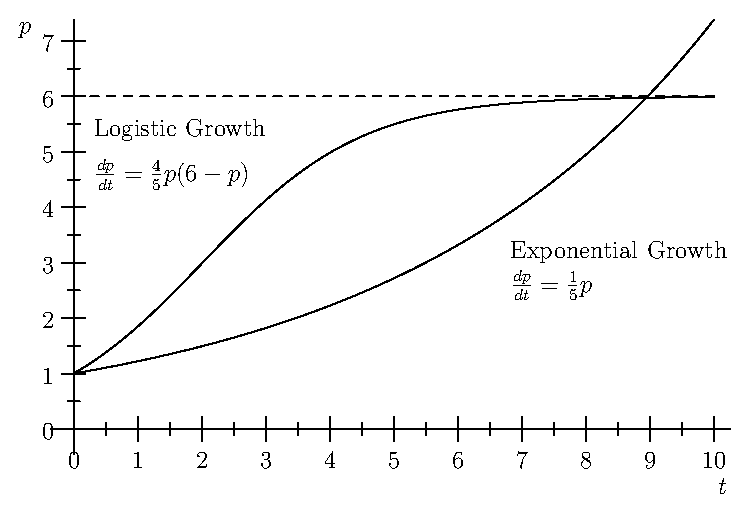
\includegraphics[width=12cm]{figure44.eps}
\caption{Exponential and Logistic Growth}
\label{Exponential and Logistic Growth}
\end{figure}

\begin{example}
\begin{equation*}
\frac{dp}{dt} = p^3 -7p^2 + 10p
\end{equation*}
The right side factors as $p(p-2)(p-5)$, so it is zero then
$p=0$, $p=2$ or $p=5$. Those are the
steady states. When $p \in (0,2)$ the derivative is positive,
so the trajectory is increasing. When $f \in (2,5)$, the
derivative is negative, so the trajectory is decreasing. When
$p \in (5,\infty)$, the derivative is positive, so the
trajectory is increasing. 
\end{example}

\begin{figure}[ht]
\centering
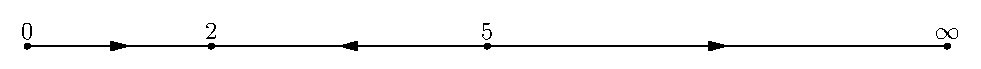
\includegraphics[width=12cm]{figure42.eps}
\caption{The Phase Line Diagram for $\frac{dp}{dt} = p^3 -
7p^2 + 10p$}
\label{Phase Line 3}
\end{figure}

\chapter{Two Motivating Problems}
\label{Two Motivating Problems}

\section*{The Velocity Problem}

\begin{figure}[ht]
\centering
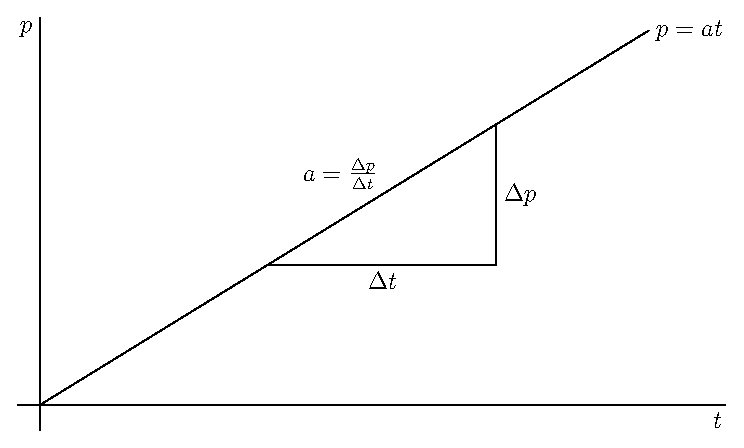
\includegraphics[width=10cm]{figure10.eps}
\caption{Slope of a Linear Function}
\label{Slope of a Linear Function}
\end{figure}

Moving from biological examples to physics, the velocity
problem is one of the basic motivating problems of calculus.
Assume we have an object moving in one dimension. We describe
its position as a function $p(t)$ where $p$ is position in
terms of time $t$. We want to know its velocity.

If $p(t) = at + b$ is a linear function, then algebra can
answer this question. With this linear function, for each
unit of time we gain $a$ units of distance. The value $a$ is
the velocity. Geometrically, the velocity is measured by the
slope of the straight line graph of $p(t)$. The slope is
measured by the ratio of the change in $p$, $\Delta p$, to the
change in $t$, $\Delta t$.

If slope is the way to measure velocity, then we need a notion
of slope for non-linear functions as well. The notion comes
from the idea of tangent lines. A tangent line to a graph is
a line which touches the graph at one point without crossing
it (as opposed to a secant line, which crosses the graph
twice).

\begin{figure}[ht]
\centering
\begin{subfigure}{.5\textwidth}
 \centering
 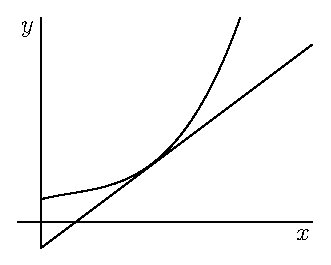
\includegraphics{figure11.eps}
 \caption{A Tangent Line}
\end{subfigure}%
\begin{subfigure}{.5\textwidth}
 \centering
 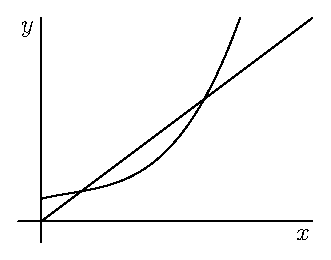
\includegraphics{figure12.eps}
 \caption{A Secant Line}
\end{subfigure}
\caption{Tangent and Secant Lines}
\label{Tangent and Secant Lines}
\end{figure}

The slope of a graph is defined to be the slope of its
tangent, should such a line exist. The velocity problem is
reduced to the problem of finding the tangent line (or, more
particularly, its slope). How do we find a tangent line?
Again, algebra has trouble with this.  The best that algebra
can do is find secant lines which approximate a tangent line.
We adjust the approximation by letting the two points of the
secant line come closer and closer together, as in the Figure
\ref{Secant Approximations 1}. In this way, we build an
approximation process which can get better an better. However,
algebra an never finish the process -- it can just supply
improved approximations.

\begin{figure}[ht]
\centering
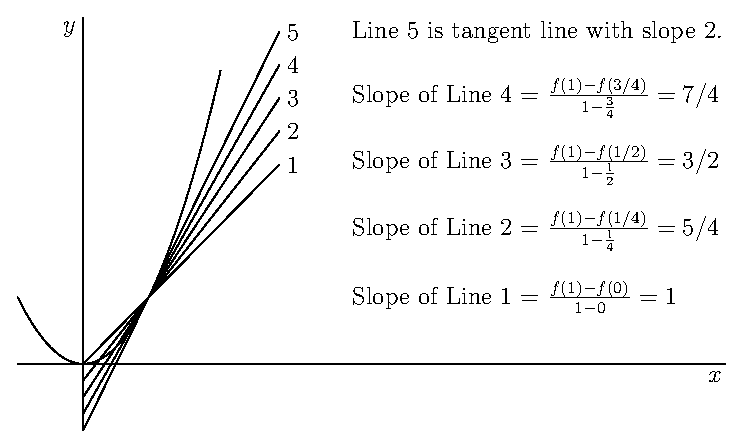
\includegraphics[width=12cm]{figure13.eps}
\caption{Secant Approximations to the Tangent Line}
\label{Secant Approximations 1}
\end{figure}

\section*{The Distance Travelled Problem}

Let's consider the opposite problem. Say we have a function
$v(t)$ which tells us the velocity of an object at any point
of time. Can we determine the distance the object has covered
over a period of time? 

\begin{figure}[ht]
\centering
\begin{subfigure}{.5\textwidth}
 \centering
 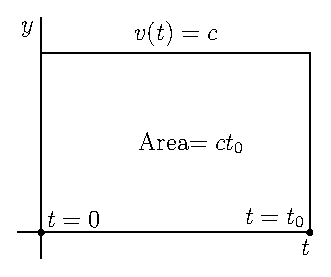
\includegraphics[width=5cm]{figure14.eps}
 \caption{Constant Velocity}
\end{subfigure}%
\begin{subfigure}{.5\textwidth}
 \centering
 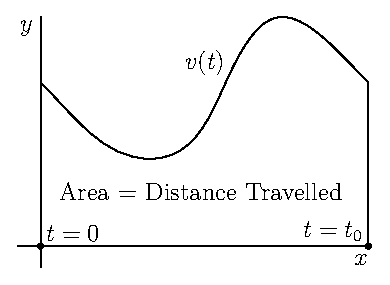
\includegraphics[width=5cm]{figure15.eps}
 \caption{Non-Constant Velocity}
\end{subfigure}
\caption{Distance Travelled Problem}
\label{Distance Travelled 1}
\end{figure}

Again, algebra can only answer this
question for very simple situations. Let's assume that
velocity $v(t) = c$ is constant. In this case, if we have
constant velocity of $c$ unit distance for unit time and we
have travelled for $t_0$ units of time, the distance is just the
product $ct_0$. Graphically, the situation is summarized in 
Figure \ref{Distance Travelled 1}. We can see that the distance
travelled under constant velocity is the area under the
velocity graph.  To solve the distance travelled problem, we
have to find areas under curves. Like tangent lines, this is
not a problem that algebra can easily tackle. However, it can
approximate areas. Algebra is good at areas of rectangles, so
we can use rectanges to approximate areas.

\begin{figure}[bt]
\centering
\begin{subfigure}{.5\textwidth}
 \centering
 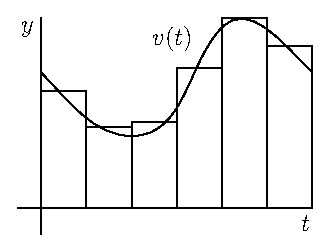
\includegraphics[width=5cm]{figure16.eps}
 \caption{Approximation of Area by Rectangles}
\end{subfigure}%
\begin{subfigure}{.5\textwidth}
 \centering
 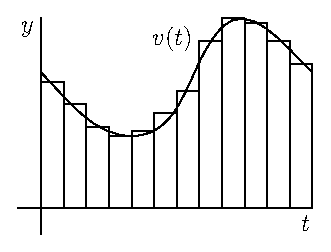
\includegraphics[width=5cm]{figure17.eps}
 \caption{Improved Approximation with More Rectangles}
\end{subfigure}
\caption{Approximating Areas under Curves}
\label{Approximating Areas under Curves 1}
\end{figure}

The sum of the areas of all the rectangles is reasonable
approximation to the area under the curve. If we want a
better approximation, we can divide into smaller rectangles.
In this way, we set up an approximation process to understand
areas under curves. Algebra can never completely answer the
question, but it can get better and better approximations by
using more and more rectangles in its approximation.

\chapter{Limits at Finite Values}
\label{Limits af Finite Values}

In the prevous section, the two motivating problems of
velocity and distance-travelled led us to approximation
processes. Inside the field of algebra, we couldn't get exact
answers to these problems, only approximate answers. 
However, algebra found a process for refining the approximation. 

Calculus starts by asking if we can somehow calculate the end
of an approximation processs. Is there an exact answer at the
end of all the approximation? Calclulus uses a new tool, the
limit, to find such an exact answer. A limit is a way of
understanding an infinite process and asking where the process
eventually leads.  The limit is the key new tool that
transcends algebra and creates calculus.

\section*{Defining Limits}

Our definition of limits will be restricted to limits of
functions. In a limit, we are comparing the input and output
of a function during an approximation process. The process
starts with moving the input towards a specific value and
observing what happens to the output.

Let $f(x)$ be a function and $a$ a point either in the domain
of the function or on the boundary of its domain. Then the
statement 
\begin{equation*}
\lim_{x \rightarrow a} f(x) = L
\end{equation*}
means that as $x$ (the input) gets closer and closer to $a$,
f(x) (the output) gets closer and closer to $L$. If such an
$L$ exists, we say the limit of $f(x)$ exists at $x=a$; we
also say that the limit converges. Otherwise we say the limit
diverges. 
\clearpage

\begin{figure}[ht]
\centering
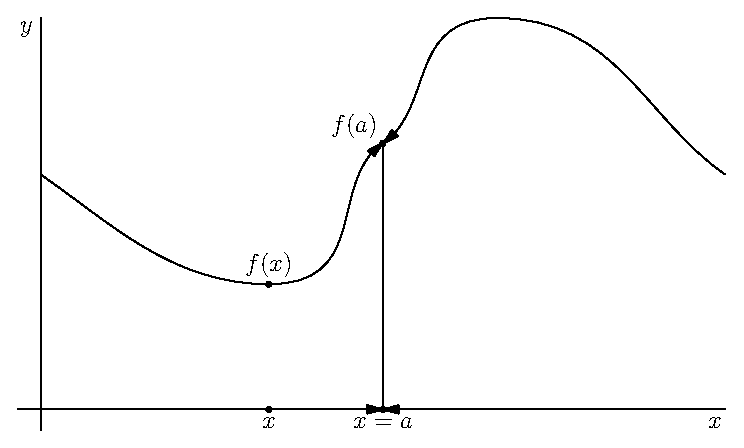
\includegraphics[width=10cm]{figure18.eps}
\caption{A Convergent Limit}
\label{A Convergent Limit}
\end{figure}

There are several ways in which the limit can diverge. The
statement
\begin{equation*}
\lim_{x \rightarrow a} f(x) = \infty
\end{equation*}
means that as $x$ gets closer and to $a$, the function value
$f(x)$ gets larger and larger without bound. The statement
\begin{equation*}
\lim_{x \rightarrow a} f(x) = -\infty
\end{equation*}
means that as $x$ gets closer and to $a$, the function value
$f(x)$ becomes a larger and larger negative value without
bound. The statement
\begin{equation*}
\lim_{x \rightarrow a} f(x) \hspace{1cm} \text{DNE}
\end{equation*}
means that the limit does not exist; it doesn't approach any
number at all.

\section*{Vertical Asymptotes}

For limits which approach $\pm \infty$, we see that the graph
of the function approaches a verticle line.  These lines are
called \emph{vertical asymptotes} for the functions.  Vertical
asymptotes are shown as the dotted lines in the Figure
\ref{Three Divergent Limits}.
\clearpage

\begin{figure}[ht]
\centering
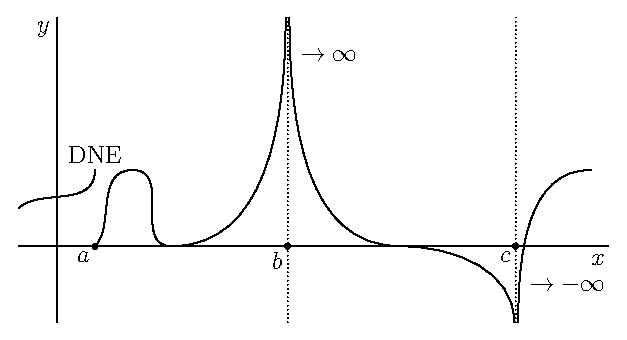
\includegraphics{figure19.eps}
\caption{Three Divergent Limits}
\label{Three Divergent Limits}
\end{figure}

\section*{One-Sided Limits}

In the above definitions, we assume that $x \rightarrow a$
means $x$ approaches $a$ from both sides, considering $x$ slightly
larger and $x$ slightly smaller than $a$. Sometimes it is
convenient to only use one side. These are called one sided
limits. If we want to approach from the left (from $x$
slightly smaller than $a$), we adjust the limit notation
slightly by writing $a^-$..
\begin{equation*}
\lim_{x \rightarrow a^-} f(x)
\end{equation*}
If we want to approach from the right (from $x$ slightly
larger than $a$), we write $a^+$. 
\begin{equation*}
\lim_{x \rightarrow a^+} f(x)
\end{equation*}

\section*{Calculating Limits}

There is a three step procedure to calculating limits.
\begin{smallitemize}
\item First, try to evaluate the function at the limit point.
For reasonable funciton (specifically, continuous funcitons,
which will be defined later), if the function can be evaluated
directly, the function value will be your limit value.
\item If the first method fails, try to work out logically
what the limit should do. 
\item If both methods fail, the limit is called an
\emph{indeterminante form}. In this case, we need to use
various algebraic tricks (factoring, expanding, multiplying by
conjugates, trig identities) and rules for manipulating limits
to change the limit into a more approachable form.
\end{smallitemize}

\section*{Limits Rule}

The third step referred to the rules for manipulating limits,
which we will now state.
Let $f$ and $g$ be functions with limits defined at $x=a$ and
let $c$ be a constant. (In the quotient limit, assume $g(x)
\neq 0$, and in the exponential limit, assume $f(x) > 0$.)
\begin{align*}
\lim_{x \rightarrow a} f(x) + g(x) & = 
\lim_{x \rightarrow a} f(x) + 
\lim_{x \rightarrow a} g(x) \\
\lim_{x \rightarrow a} f(x) - g(x) & = 
\lim_{x \rightarrow a} f(x) - 
\lim_{x \rightarrow a} g(x) \\
\lim_{x \rightarrow a} c f(x) & = 
c \lim_{x \rightarrow a} f(x) \\
\lim_{x \rightarrow a} f(x) g(x) & = 
\lim_{x \rightarrow a} f(x) 
\lim_{x \rightarrow a} g(x) \\
\lim_{x \rightarrow a} \frac{f(x)}{g(x)} & = 
\frac{\lim_{x \rightarrow a} f(x)}
{\lim_{x \rightarrow a} g(x)} \\
\lim_{x \rightarrow a} (f(x))^c & = 
(\lim_{x \rightarrow a} f(x))^c 
\end{align*}
In addition to the limit rules, there are two limits that are
frequently useful.  The second limit can be taken as a
definition of the exponential base $e$. 
\begin{align*}
\lim_{x \rightarrow 0} \frac{\sin x}{x} & = 1 \\
\lim_{x \rightarrow 0^+} \left( 1 + x \right)^{\frac{1}{x}} & = e
\end{align*}

\chapter{Limits at Infinity and Asymptotic Analysis }
\label{Limits at Infinity}

\section*{Definition of Limits at Infinity}

In addition to asking what happens to a function as the input
approaches paticular finite values, we can also ask what
happens as the input approaches infinity, that is, at the
input gets larger and larger. 

The statement
\begin{equation*}
\lim_{x \rightarrow \infty} f(x) = L
\end{equation*}
means that as $x$ gets larger and larger without bound, $f(x)$
gets closer and closer to $L$. The statement
\begin{equation*}
\lim_{x \rightarrow \infty} f(x) = \infty
\end{equation*}
means that as $x$ gets larger and larger without bound, $f(x)$
also gets larger and larger without bound. The statement 
\begin{equation*}
\lim_{x \rightarrow \infty} f(x) = -\infty
\end{equation*}
means that as $x$ gets larger and larger without bound, $f(x)$
becomes a larger and larger negative number without bound.

These statements are defined the same way for $x \rightarrow
-\infty$ when $x$ becomes a larger and larger negative number
without bound.

\begin{figure}[ht]
\centering
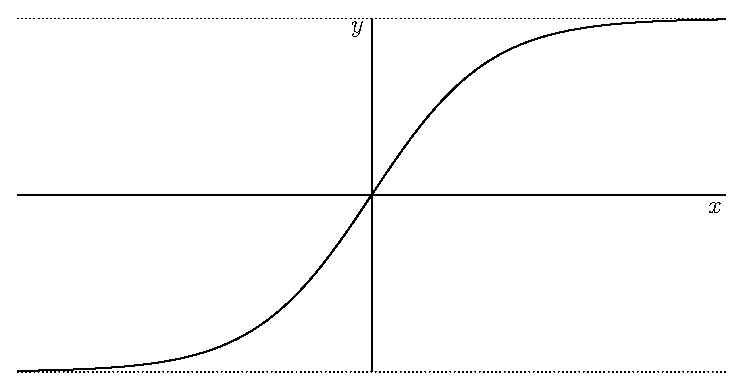
\includegraphics[width=10cm]{figure20.eps}
\caption{Horizontal Asymptotes}
\label{Horizontal Asymptotes}
\end{figure}

\section*{Horizontal Asymptotes}

If we have a function $f(x)$ where the limit 
\begin{equation*}
\lim_{x \rightarrow \pm \infty} f(x) = L
\end{equation*}
exists either at positive or negative infinity, that means
that the graph of the function approaches the line $y=L$.
Such lines are called \emph{horizontal asymptotes}.

\section*{Calculation of Infinite Limits}

The calculation of infinite limits is similar to the same
steps as finite limits except that the first step, evaluation,
is impossible. We start at the second step and look for a
simple logical explanation. If such an explanation is not
forthcoming, the limit is an indeterminate form and we use
algegra and the limit rules. The limit rules apply to infinite
limits as they did to finite limits.

\section*{Asymptotic Analysis}

In addition to the algebraic methods already discussed, for
infinite limits there is a powerful technique called
asymptotic analysis. In practice, this is the most commonly
used approach to infinite limits.

Asymptotic analysis interprets limit at infinity
as a measurement of the growth of functions. The functions
$f_1(x) = x$, $f_2(x) = x^2$ and $f_3(x) = e^x$ all get very large as
$x$ gets very large; they all grow. Asymptotic analysis asks
which of these functions grows faster. 

The limit of a ratio of function $\frac{f(x)}{g(x)}$ is asking
essentially the same question. By looking at the ratio of two
functions as $x \rightarrow \infty$, we ar implicitly asking
which grows faster. If $g$ grows faster, then the denominator
should outpace the numerator, and the limit should tend to
$0$. If $f$ grows faster, then the numerator should outpace
the denominator and the limit should tend to $\infty$. If $f$
and $g$ has roughly the same growth, then the limit should
settle to some finite value larger than $0$. This leads to
the notion of asymptotic order.

\section*{Asymptotic Order}

In asymptotic analysis, we start with a quotient limit.
\begin{equation*}
\lim_{x \rightarrow \pm \infty} \frac{f(x)}{g(x)}
\end{equation*}
\begin{itemize}
\item If this limit is $0$, then we say that $g$ has greater
asymptotic order than $f$. Alternatively, we say that $g$ grows
faster than or $g$ dominates $f$ as $x \rightarrow \infty$. 
\item If this limit is $\infty$, then we say that $f$ has
greater asymptotic order than $g$. Alternatively, we say that
$f$ grows faster than or $f$ dominates $g$.
\item If this limit is finite but non-zero, we say that $f$ and
$g$ have the same asymptotic order. Alternatively, we say that
$f$ and $g$ grow at the same asymptotic rate and neither
dominates.
\end{itemize}
With this definition, we can evaluate many limits by just
knowing which functions have greater or lesser asymptotic
order.

\section*{An Asymptotic Ranking of Functions}

Here are several rules for asymptotic order of functions. Many
of these are obvious, but some require more work to establish.
The proofs of these statements are not included in this
course.
\begin{itemize}
\item A constant function $f(x) = c$ has a lower asymptotic
order than any increasing function.
\item Any multiple of a function $c f(x)$ has the same
asymptotic order as the original function $f(x)$. 
\item The logarithm $f(x) = \ln x$ grows slower than any
function $f(x) = x^r$ for $r > 0$. 
\item The function $f(x) = x^r$ grows slower than $g(x) = x^s$
as long as $0 < r< s$. In particular, polynomials of lower
degree grow slower than polynomials of higher degree.
\item The exponential function $f(x) = e^x$ grows faster than
$g(x) = x^r$ for any $r$.
\item The function $f(x) = x^x$ grows faster than $g(x) = e^x$.
\end{itemize}
These are the most common types of functions we will consider.
We can summarize this in a list of asymptotic orders: in the
following list `$f<g$' means that $f$ grows slower
than $g$. 
\begin{equation*}
c < \ln x < \ldots < x^{\frac{1}{3}} < x^{\frac{1}{2}} < x < x^2
< x^3 < \ldots < e^x < x^x < \ldots
\end{equation*}
This is the basic list and is something you will either
memorize or frequently reference for many limits in this course.
There are other functions at the top of this list which grow
faster than $x^x$, but they are not frequently used.

\section*{Determining Asymptotic Order}

In quotient limits, $f$ and $g$ may be more complicated than
the simple functions in our asymptotic ranking. We have a
two useful rules to help us work with $f$ and $g$ which are
combinations of pieces of various asymptotic order.
\begin{itemize}
\item If $f = f_1 + f_2 + f_3 + \ldots + f_n$ then the
asymptotic order of $f$ is the maximum of the asymptotic order
of the $f_i$. This means that in a sum or difference, we only
need to consider the fastest growing pieces. We can simply
ignore all the rest.
\item If $f_1 < g_1$ and either $f_2 < g_2$ or $f_2$ and $g_2$
have the same asymptotic order, then $f_1 f_2 < g_1 g_2$.
Basically, this says that relationships of asymptotic order are
preserved in products.
\end{itemize}

\section*{Ratios with Equivalent Asymptotic Order}

In a quotient limit where $f$ and $g$ have the same asymptotic
order, we look at the \emph{leading coefficients}. The leading
coefficients are the coefficients which sit in front of the
term with the highest asymptotic order. 

\begin{example}
\begin{equation*}
\lim_{x \rightarrow \infty} \frac{8x^4 + 3x^2 + 4}{14x^4 -
9x^3 - 50x^2 - 4x - 1}
\end{equation*}
The leading coefficient in the numerator if $8$, and in the
denominator is $14$. Only these terms matter, which radically
simplifies the limit
\begin{equation*}
\lim_{x \rightarrow \infty} \frac{8x^4 + 3x^2 + 4}{14x^4 -
9x^3 - 50x^2 - 4x - 1} = \frac{8}{14} = \frac{4}{7}
\end{equation*}
Note that none of the information associated to the pieces of
lower asymptotic order matters at all. No matter how large
the constants may be, only the asymptotic order tells us which
pieces are important.
\end{example}

\chapter{Limits, Asymptotics and Models}
\label{Limits, Asymptotics and Models}

We can use our tools of limits and asymptotic analysis to
analyze models. Limits at finite values tell us how models
behave near their undefined points; in particular, whether
they diverge to infinity or remain bounded. This leads to an
understanding of the limitations of a model and how it behaves
at its own extreme situations.

Limits at infinity and asymptotic analysis tells us about the
growth and long term behaviour of a model. We can compare
population growth models asymptotically to get an idea of
which is fundamentally a faster growth model. The analysis of
algorithms in computing science is also done almost entirely
with asymptotic analysis; the asymptotic order of an algorithm
is a very good measure of how fast it can operate. 

The notion of \emph{stability} is frequently the focus of our
study of limits and models. The word `stability' has various
technical definitions in pieces of applied mathematics, but it
always relates to the limits of the model and the behaviour
near those limits. 

If we consider popluation models, we have four categories of
long term (asymptotic) behaviour. 
\begin{smallitemize}
\item The function can grow without bound, as in the
exponential growth function $p(t) = p_0 e^{at}$.
\item The function can decay to zero, as in the exponential
decay function $p(t) = p_0 e^{-at}$.
\item The function can approach a steady state, as in the
logistic growth function 
\begin{equation*}
p(t) = \frac{p_0 K e^{at}}{K + p_0 (e^{at}-1)}
\end{equation*}
\item The function can osscilate without ever reaching a
steady state, possibly with chaotic behaviour. A non-chaotic
osscilating function is this periodic version of logistic
growth:
\begin{equation*}
p(t) = \left(\frac{p_0 K e^{at}}{K + p_0 (e^{at}-1)} \right)
\left( 1 + \frac{1}{5} \sin (bt) \right) 
\end{equation*}
\end{smallitemize}

Asymptotic analysis can also give information about the
extreme values in a model. Consider the ideal gas law (where
$P$ is pressure, $V$ is volume, $n$ is the amount of gas, $T$
is temperature and $R$ is a constant. (We assume that $P$ and
$V$ are the variables, and $n$, $R$ and $T$ are constant.)
\begin{equation*}
PV = nRT
\end{equation*}
We can ask what happens to pressure at low volumes, expressed
as a limit as $V \rightarrow 0$.
\begin{equation*}
\lim_{V \rightarrow 0} P = \lim_{V \rightarrow 0}
\frac{nRT}{V} = \infty
\end{equation*}
This tells us that low volumes result in high pressures.
We could equivalently ask what happens at very high
volumes.
\begin{equation*}
\lim_{V \rightarrow \infty} P = \lim_{V \rightarrow \infty}
\frac{nRT}{V} = 0
\end{equation*}
Unsurprisingly, very large volume result in very low
pressures.

The behaviour at extreme values depends on the particulars of
the models. A more complicated gas law is the Vander Waal's
gaw law (where $a$ and $b$ are new positive constants).
\begin{equation*}
\left( P + \frac{n^2 a}{V^2} \right) \left( V - nb \right) =
nRT
\end{equation*}
What happens for these gasses at high pressures? It's
difficult to solve directly for volume, but we can analyze the
equation in its current form. If the term involving pressure
grows very large, the term only involving volume must grow to
zero, so that the product remains the same. That happens when
$V$ is very close to the value $nb$.
\begin{equation*}
\lim_{P \rightarrow \infty} V = nb
\end{equation*}
Therefore, in this model, extreme pressures happen near the
fixed, but non-zero, volume $V = nb$.

\chapter{Continuity}
\label{Continuity}

\begin{figure}[ht]
\centering
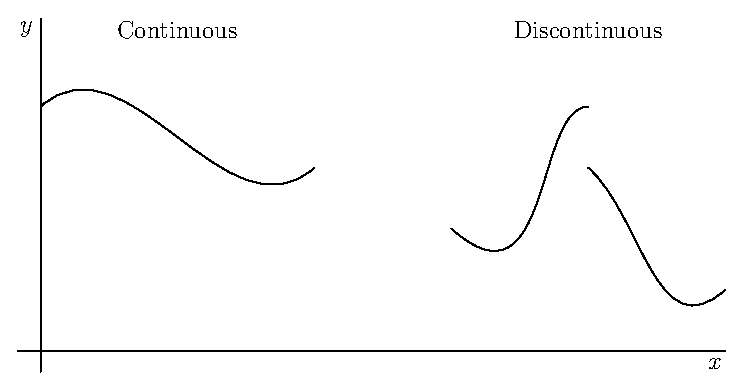
\includegraphics[width=12cm]{figure45.eps}
\caption{Continuity}
\label{Continuity Diagram}
\end{figure}

A function is continuous at a point $a$ in its domain if 
\begin{equation*}
f(a) = \lim_{x \rightarrow a} f(x)
\end{equation*}

We have already encounted these kinds of limit: in the
calculation of limits, the first step was to try to evaluate
the function at the limit point. We were implicitly relying
on the continuity of our standard functions. Happily, 
we were justified in doing so: all the standard elementary
functions (polynomials, rational function, algebraic
functions, trig, exponentials) are continuous on their
domains. The phrase `on their domains' is important; where
there is a break in the domain, the function cannot be
continuous. Continuity only happens inside the domain of a
function.  Visually, the graph of a continuous function is
connected; it can be drawn without lifting your pen (pencil,
chalk, etc).

\section*{Intermediate Value Theorem}

Though it has a formal name, the Intermediate Value Theorem is
a very sensible and obvious result of continuity. Formally
stated, the theorem says that if $f$ is a continuous function
on an interval $[a,b]$ and $\alpha$ is a real number with
$f(a) < \alpha < f(b)$ or $f(a) > \alpha > f(b)$, then there
exists a number $c \in (a,b)$ such that $f(c) = \alpha$. 

Rephrased, the theorem says that a continuous function cannot
skip any values. If $f(a) = 0$ and $f(b) = 1$, then the
function must output all values between $0$ and $1$ as the
input goes from $a$ to $b$. Continuity means the graph is
connected; it can't jump over any intermediate values.

\begin{figure}[t]
\centering
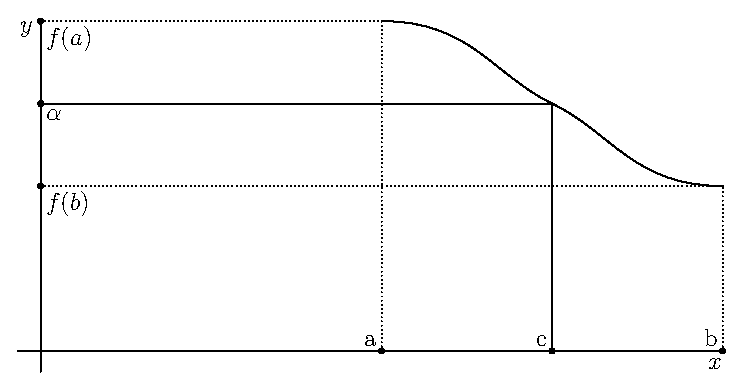
\includegraphics[width=12cm]{figure46.eps}
\caption{Intermediate Value Theorem}
\label{Intermediate Value Theorem}
\end{figure}

\section*{Piecewise Functions}

We know that all of our familiar elementary functions are
continuous on their domains. One might ask why we are worried
about continuity at all? A common place where continuity
becomes an issue is in piecewise functions. These are
functions which have different expressions or definitions over
different pieces of their domain. There is a particular
notation for piecewise functions. Say we have a function on
$\RR$ which has two definitions, one for $x<a$ and another $x
\geq a$. Then the function is written
\begin{equation*}
f(x) = \left\{ \begin{matrix} g(x) & x < a \\ h(x) & x \geq a
\end{matrix} \right.
\end{equation*}

\begin{figure}[ht]
\centering
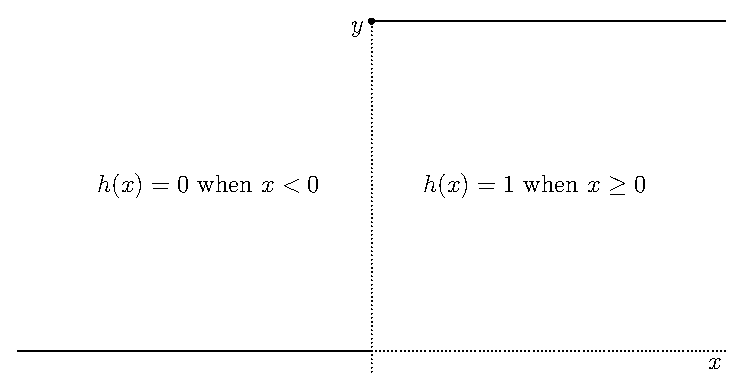
\includegraphics[width=12cm]{figure21.eps}
\caption{The Heaviside Function}
\label{The Heaviside Function}
\end{figure}

A very well-known example is the Heaviside function.
\begin{equation*}
f(x) = \left\{ \begin{matrix} 0 & x < 0 \\ 1 & x \geq 0
\end{matrix} \right.
\end{equation*}
The Heaviside function is very frequently used to model
switches: it suddenly changes from off (0) to on (1) at $x=0$.
This is a discontinuous change, as the function jumps from $0$
to $1$ without going through any intermediate value.

In the definition of a piecewise function, there can be more
than two pieces and the conditions on $x$ can be more
complicated than inequalities. Here is a piecewise function
with three pieces defined on intervals.
\begin{equation*}
f(x) = \left\{ \begin{matrix} 
x^2 -1 & x \in (-5,0) \\
x^2 + 1 & x \in [0,3] \\
3x-5 & x \in (3,7) 
\end{matrix} \right.
\end{equation*}
The domain of this function is $(-5,7)$, which is the union of
all the intervals of definition in the piecewise expression.
It's graph is Figure \ref{A Discontinuous Piecewise Function}.

Piecewise functions can be extremely strange.
\begin{equation*}
f(x) = \left\{ \begin{matrix} 1 & x \in \QQ \\ 0 & x \notin
\QQ \end{matrix} \right.
\end{equation*}
This function depends on whether its input is rational or
irrational, returning one and zero respectively. It is a
horendously discontinuous functions, with ones and zeros
everywhere and no intermediate values. 
\clearpage

\begin{figure}[ht]
\centering
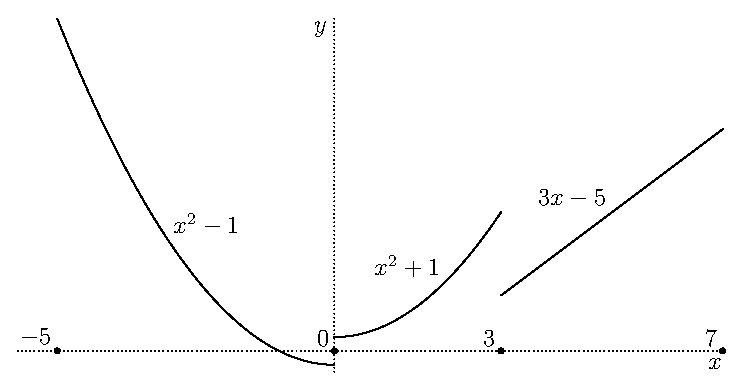
\includegraphics[width=12cm]{figure47.eps}
\caption{A Discontinuous Piecewise Function}
\label{A Discontinuous Piecewise Function}
\end{figure}

\section*{Continuity of Piecewise Functions}

It is important to be able to check if a piecewise function is
continuous at its crossover point. Say we have a piecewise
function with a break at $x=a$.
\begin{equation*}
f(x) = \left\{ \begin{matrix} g(x) & x < a \\ h(x) & x \geq a
\end{matrix} \right.
\end{equation*}
It is natural to ask if $f$ is continuous at $x=a$. In order
to investigate this, we need to look at the function value and
the limits from both sides. The function is continuous if all
three are the same.
\begin{equation*}
\lim_{x \rightarrow a^-} f(x) = 
\lim_{x \rightarrow a^+} f(x) = f(a)
\end{equation*}

\chapter{Definition of the Derivative}
\label{Definition of the Derivative}

\section*{Limits of Secant Line}

\begin{figure}[ht]
\centering
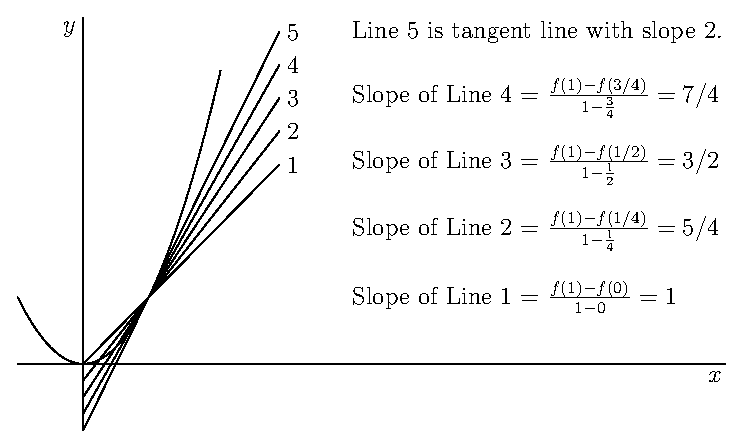
\includegraphics{figure13.eps}
\caption{Secant Approximations to the Tangent Line}
\label{Secant Approximations 2}
\end{figure}

In Section \ref{Population Growth}, we defined the derivative
as the rate of change of a function. In Section \ref{Two
Motivating Problems}, we
connected that definition to the geometry of slopes of tangent
lines and constructed a process by which algebra can
approximate a tangent line by using secant lines. Now that we
have limits, we can ask for the limit of that approximation
process.

Let's say we want the slope of the tangent line at a point
$(a,f(a))$ on the graph of a function. We can take $a$ as
one point to define a secant line and let $x$ be the other
point (with $x \neq a$). Then the slope of the secant line is
the difference in output ($f(x) - f(a)$) dividing by the
difference in input ($x-a$). 
\begin{equation*}
\frac{f(x) - f(a)}{x-a}
\end{equation*}
We said that we should get better and better approximations to
the tangent line as $x$ gets closer to $a$. Now we can ask
for the limit as $x \rightarrow a$.
\begin{equation*}
\lim_{x \rightarrow a} \frac{f(x) - f(a)}{x-a}
\end{equation*}
This limit, if it exists, will be the slope of the tangent
line. It is called the derivative and is the rate of change
of the function at $x=a$.
\begin{equation*}
f^\prime(a) = \frac{df}{dx} (a) = \lim_{x \rightarrow a}
\frac{f(x) - f(a)}{x-a} 
\end{equation*}
There is a slight alteration of the definition, which is
useful for some calculations. If we let $h = x-a$, then we can
write the limit as:
\begin{equation*}
f^\prime(a) = \frac{df}{dx} (a) = \lim_{h \rightarrow 0}
\frac{f(a+h) - f(a)}{h} 
\end{equation*}
This second definition allows us to see that the derivative is
an entirely new function. At each point $x$ in the
domain of $f$, we can ask for the slope of the tangent line.
That gives a new function:
\begin{equation*}
f^\prime(x) = \frac{df}{dx} = \lim_{h \rightarrow 0}
\frac{f(x+h) - f(x)}{h} 
\end{equation*}

\section*{Differential Operators}

We think of the derivative as an operation on functions: it
takes a function and gives us a new function which measures
the rate of change of the previous function. This solves the
velocity problem: if $x(t)$ is a position function, then its
derivative $x^\prime(t)$ is the velocity function. 

Leibniz notation is useful for thinking of derivatives as
operators. If we seperate the notation slightly, we can write
\begin{equation*}
\frac{df}{dx} = \frac{d}{dx} f
\end{equation*}
With this notation, we think of $\frac{d}{dx}$ as the
operator: the thing that takes derivatives. Having notation
for such an operator is extremely convenient.

\section*{Differentiability}

The limit defining the derivative may not always exist. If it
does exist at a point $a$ in the domain, we say that $f$ is
\emph{differentiable} at the point $a$. If it exists for all points
in the domain of $f$, we say that $f$ is a differentiable
function. Differentiability requires continuity: if a
function makes a sudden jump, it doesn't make sense to talk
about a rate of change and a tangent line cannot be defined.
Differentiability also requires a `smoothness' condition. A
function whose graph has sharp corners is not differentiable
at the sharp corners, because it doesn't make sense to define
a tangent line at a sharp corner. The graph of the function
must be smooth. Figure \ref{Differentiability Problems}  shows
how a jump or sharp corner makes the choice of a tangent line
problematic.

\begin{figure}[t]
\centering
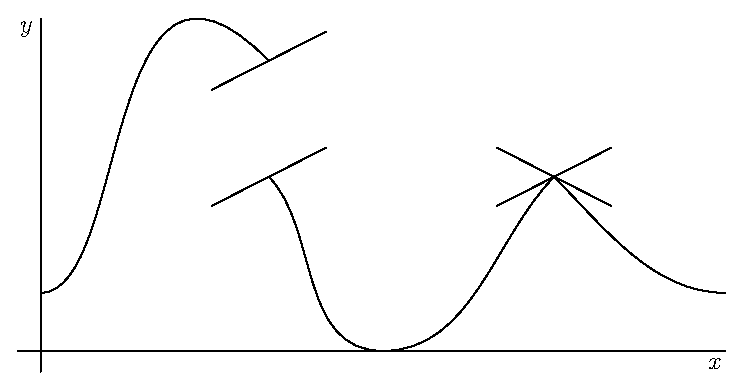
\includegraphics[width=12cm]{figure48.eps}
\caption{Differentiability Problems}
\label{Differentiability Problems}
\end{figure}

\section*{Interpretation}

Now that we have a definition of the derivative and
differentiability, let's review what this all means. The
derivative has two major interpretation, one geometric and one
applied. 
\begin{itemize}
\item The derivative measures the slope of a tangent line to a
function.
\item The derivative measures the rate of change of a function.
\end{itemize}
If a function is differentiable on its domain, that means its
derivative exists at all points in the domain. In the
geometric interpretation, this means that the graph of the
function has a well-defined tangent line at all points in its
domain. In the applied interpretation, this means that the
function has a well-defined rate of change at all points in
its domain.

\chapter{Derivative Rules Part 1}
\label{Derivative Rules Part 1}

Now that we have the definition and an idea of its meaning, we
move on to several lectures on the technical details of
calculating derivatives. 

\section*{Important Derivatives}

We'll start with a number of standard derivatives. If a
function is constant, its rate of change is zero, so its must
have a zero derivative. 
\begin{equation*}
\frac{d}{dx} c = 0
\end{equation*}
For the function $f(x) = ax + b$, the graph is a straight line
with slope $a$. Since the derivative measures the slope, it
should be constant $a$.
\begin{equation*}
\frac{d}{dx} ax + b = a
\end{equation*}
We have two standard derivatives we start with for
trigonometry. There are given here without proof.
\begin{equation*}
\frac{d}{dx} \sin x = \cos x \quad \quad \hspace{2cm}
\frac{d}{dx} \cos x = -\sin x \quad \quad 
\end{equation*}
We also have a standard derivative for the exponential
function, established  using the definition of the
derivative.
\begin{align*}
\frac{d}{dx} a^x & = \lim_{h \rightarrow 0} \frac{a^{x+h} -
a^x}{h} = \lim_{h \rightarrow 0} \frac{a^x a^h - a^x}{h} \\
& = \lim_{h \rightarrow 0} a^x \frac{a^h-1}{h} = 
= a^x \lim_{h \rightarrow 0} \frac{a^h-1}{h} = 
a^x \left( \left. \frac{d}{dx} a^x \right|_{x=0} \right) 
\end{align*}
In the last step, we changed the limit into a derivative using
the definition of the derivative at the specific point $x=0$.
The vertical line means ``evaluated at $x=0$''. 

This formula shows that derivative of $a^x$ is formed by
multiply by the derivative at $x=0$. Note that all
exponentials go through the point $(0,1)$. Figure \ref{Four
Exponential Functions} shows the the graphs of several
exponential function (for bases $a > 1$).

\begin{figure}[t]
\centering
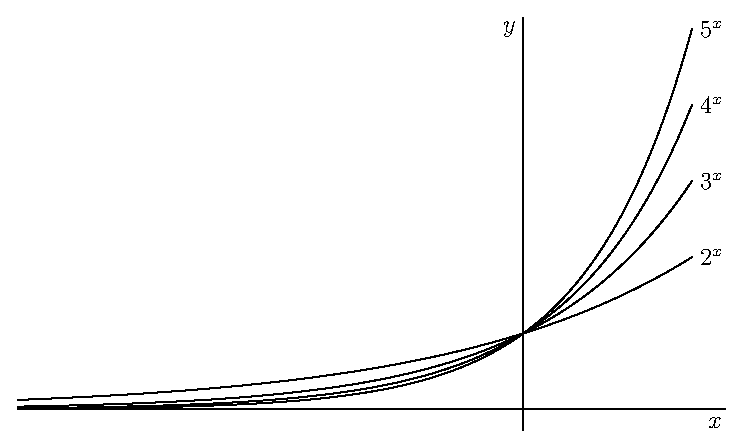
\includegraphics[width=10cm]{figure49.eps}
\caption{Four Exponential Functions}
\label{Four Exponential Functions}
\end{figure}

The slope at $(0,1)$ determines
the derivative. As seen in the Figure \ref{Four Exponential
Functions}, for different
choices of the base, we get different slopes going through the
point $(0,1)$. There is one special base which has slope $1$ at the
point $(0,1)$. By definition, that base is the number $e$.
(This number was defined earlier by a limit and we in Calculus
II that the two definitions coincide.) By definition, the
function $e^x$ satisfies an important property.
\begin{equation*}
\frac{d}{dx} e^x = e^x
\end{equation*}
This is the main reason that we are so fond of $e$ as an
expoenntial base. $e^x$ is the nicest function to
differentiate, since it doesn't change at all. 

\section*{Power Rule}

So far, we've looked at specific derivatives and used the
definition to work them out. This approach quickly becomes
intenable due to complications in the limit calculation.
Therefore, we'd like to find some general rules that allow us
to calculate derivatives without using the definition. The
first rules is called the power rules. Let $n \in \RR$ with $n=0$.
\begin{equation*}
\frac{d}{dx} x^n = nx^{n-1} 
\end{equation*}
We can give a proof when $n$ is a positive integer, using the
binomial theorem.
\begin{align*}
\frac{d}{dx} x^n & = \lim_{h \rightarrow 0} \frac{(x+h)^n -
x^n}{h} = \\
& = \lim_{h \rightarrow 0} \frac{x^n + nx^{n-1}h + \binom{n}{2}
x^{n-2}h^2 + \ldots + nxh^{n-1} + h^n - x^n}{h} \\
& = \lim_{h \rightarrow 0} \frac{nx^{n-1}h + \binom{n}{2}
x^{n-2}h^2 + \ldots + nxh^{n-1} + h^n}{h} \\
& = \lim_{h \rightarrow 0} nx^{n-1} + \binom{n}{2} x^{n-2}h + 
\ldots + nxh^{n-2} + h^{n-1} \\
& = nx^{n-1}
\end{align*}

\section*{Linearity}

The next rules is a set of three rules which are called
linearity. (Linearity shows that derivatives addition,
subtraction and multiplication by constants. In general, any
operation in mathematics that cooperates with those these
actions is called a linear property). If $f$ and $g$ are
differentiable functions and $c$ is a real constant, then
three rules hold.
\begin{align*}
\frac{d}{dx} f + g & = \frac{df}{dx} + \frac{dg}{dx} \\
\frac{d}{dx} f - g & = \frac{df}{dx} - \frac{dg}{dx} \\
\frac{d}{dx} cf & = c \frac{df}{dx}
\end{align*}
The proof of the linearity rules is excluded here, though it
is relatively easy to construct using the linearity of the
limit and the definition of the derivative. Using linearity
and the power rule, we can take the derivative of any
polynomial. 

\begin{example}
\begin{align*}
\frac{d}{dx} x^2 -3x -4 & = \frac{d}{dx} x^2 - \frac{d}{dx} 3x
- \frac{d}{dx} 4 = 2x - 3 - 0 = 2x -3 \\
\frac{d}{dx} 7x^3 + 9x^2 - 14x - 26 & = 7 \frac{d}{dx} x^3 + 9
\frac{d}{dx} x^2 - 14 \frac{d}{dx} x - \frac{d}{dx} 26 \\
& = 7 (3x^2) + 9(2x) - 14 - 0 = 21 x^2 + 18 x - 14 
\end{align*}
\end{example}

\section*{Leibniz Rule}

Limits worked well with all four arithmetic operations:
addition, subtraction, multiplication and division. We might
hope the same is true for derivatives, but we would be
disappointed. There are rules for multiplication and division,
but they are more complicated that what we had for limits.
The rule for products is called the product rules or the
Leibniz rule. Let $f$ and $g$ be differentiable functions.
\begin{equation*}
\frac{d}{dx} fg = g \frac{df}{dx} + f \frac{dg}{dx} 
\end{equation*}
The Leibniz rule is, in many ways, the archetypical rule that
identifies differentiation. There are many derivative-like
operations in mathematics and they all conform to some version
of the Leibniz rule. 

The following calculation is a proof for the Leibniz rule.
Note in the second step, we've added and subtracted the same
term in the numerator.
\begin{align*}
\frac{d}{dx} fg & = \lim_{h \rightarrow 0} \frac{f(x+h)g(x+h) -
f(x)g(x)}{h} \\
& = \lim_{h \rightarrow 0} \frac{f(x+h)g(x+h) - f(x+h) g(x) +
f(x+h) g(x) - f(x)g(x)}{h} \\
& = \lim_{h \rightarrow 0} f(x+h)\frac{g(x+h) - g(x)}{h} +
\lim_{h \rightarrow 0} g(x) \frac{f(x+h) - f(x)}{h} \\
& = f(x) \lim_{h \rightarrow 0} \frac{g(x+h) - g(x)}{h} +
g(x) \lim_{h \rightarrow 0} \frac{f(x+h) - f(x)}{h} \\
& = f(x) \frac{dg}{dx} + f(x) \frac{df}{dx}
\end{align*}

\begin{example}
\begin{align*}
\frac{d}{dx} x^2 e^x & = 2x e^x + x^2 e^x \\
\frac{d}{dx} x^2 \sin x & = 2x \sin x + x^2 \cos x \\
\frac{d}{dx} e^x \sin x & = e^x \sin x + e^x \cos x 
\end{align*}
\end{example}

\section*{Quotient Rule}

Let $f$ be a differentiable function
and $g$ be a differentiable function with $g(x) \neq 0$, then
the quotient rule states:
\begin{equation*}
\frac{d}{dx} \frac{f(x)}{g(x)} = \frac{\frac{df}{dx} g(x) - f(x)
\frac{dg}{dx}}{(g(x))^2}
\end{equation*}

\begin{example}
\begin{align*}
\frac{d}{dx} \tan x & = \frac{d}{dx} \frac{\sin x}{\cos x} =
\frac{\frac{d \sin x}{dx} \cos x - \sin x \frac{d \cos
x}{dx}}{\cos^2 x} = \frac{\cos^2 x + \sin^2 x}{\cos^2 x} =
\sec^2 x \\
\frac{d}{dx} \sec x & = \frac{d}{dx} \frac{1}{\cos x} = \frac{0 -
- \sin x}{\cos^2 x} = \sec x \tan x 
\end{align*}
\end{example}

\chapter{Derivative Rules Part 2}
\label{Derivative Rules Part 2}

\section*{Chain Rule}

The rules we have so far give us the tools to calculate many
derivatives. However, they don't address composition. 
How do we differentiate $\sin x^2$? The rule that
addresses derivatives of composed functions is called the chain
rule. The chain rule has two notations.  Let $f$ and $g$ be
differentiable functions and consider the composition
$f(g(x))$. It is often useful to label $g(x)$ by a new,
temporary variable $u = g(x)$. The vertical line mean evaluate
by replaing $u$ with $g(x)$.
\begin{equation*}
\frac{d}{dx} f(g(x)) = f^\prime(g(x)) g^\prime(x) = \left.
\frac{df(u)}{du} \right|_{u=g(x)} \frac{dg}{dx} 
\end{equation*}
The variety of notations is somewhat due to the difficult
nature of the rule---it's hard to clearly describe. The key
idea is to think of composition in terms of inside and outside
functions. The derivative of the composition is the derivative of the
outside ($f^\prime$) evaluted at the inside ($f^\prime(g(x))$),
then multiplied by the derivative of the inside ($g^\prime$).
There is one other way of expressing the chain rule.
\begin{equation*}
\frac{df}{dx} = \frac{df}{dg} \frac{dg}{dx}
\end{equation*}
In this last version of the chain rule, we can think of the
infinitesimals $df$, $dg$ and $dx$ as something like fractions
in Leibniz notation ($\frac{df}{dx}$). These terms are not
fractions, but they act a bit like fractions.
\clearpage

The proof of the chain rule is tricky, but the following
argument gives the idea. The argument is a little imprecise
in the fourth step, where we replace $g(x)$ with the temporary
variable $u$, since we haven't established that such an
operation is valid. In the proof, let $F = f \circ g$.
\begin{align*}
\frac{dF}{dx}(a) & = \lim_{x \rightarrow a} \frac{f \circ g (x)
- f \circ g(a)}{x-a} = \lim_{x \rightarrow a} \frac{f(g(x)) -
 f(g(a))}{x-a} \\
& = \lim_{x \rightarrow a} \frac{f(g(x)) - f(g(a))}{g(x) - g(a)}
\frac{g(x) - g(a)}{x-a}\\
& = \lim_{x \rightarrow a} \frac{f(g(x)) - f(g(a))}{g(x) - g(a)}
\lim_{x \rightarrow a} \frac{g(x) - g(a)}{x-a} \\
& = \lim_{u \rightarrow g(a)} \frac{f(u) - f(g(a))}{u - g(a)}
\lim_{x \rightarrow a} \frac{g(x) - g(a)}{x-a} \\
& = \left. \frac{df}{du} \right|_{u=g(a)} \left.
\frac{dg}{dx} \right|_{x=a} = f^\prime(g(a)) g^\prime(a)
\end{align*}

\begin{example}
\begin{align*}
\frac{d}{dx} e^{ax} & = ae^{ax} \\
\frac{d}{dx} \sin 3x & = 3 \cos 3x \\
\frac{d}{dx} e^{x^2+2} & = (2x) e^{x^2+2} \\
\frac{d}{dx} e^{e^x} & = e^x e^{e^x} \\
\frac{d}{dx} \sin \left( \frac{x^2+1}{x^2-1} \right) & = \cos
\left( \frac{x^2+1}{x^2-1} \right) \frac{d}{dx}
\frac{x^2+1}{x^2-1} \\
& = \cos \left( \frac{x^2+1}{x^2-1} \right) \frac{(x^2-1)
\frac{d}{dx} (x^2+1) - (x^2+1) \frac{d}{dx} (x^2-1)}{(x^2-1)^2} \\
& = \cos \left( \frac{x^2+1}{x^2-1} \right) \frac{(x^2-1)
(2x) - (x^2+1) (2x)}{(x^2-1)^2} \\
& = \cos \left( \frac{x^2+1}{x^2-1} \right) \frac{2x(x^2-1 - x^2
-1)}{(x^2-1)^2} = - \cos \left( \frac{x^2+1}{x^2-1} \right) 
\frac{4x}{(x^2-1)^2} \\
\frac{d}{dx} \cos ( e^{\sin x}) & = -\sin (e^{\sin x})
\frac{d}{dx} e^{\sin x} = -\sin (e^{\sin x}) e^{\sin x}
\frac{d}{dx} \sin x = -\sin (e^{\sin x}) e^{\sin x} \cos x 
\end{align*}
\end{example}

\begin{example}
We can use the chain rule to differentiate
arbitrary exponential functions in more detail than before:
\begin{align*}
\frac{d}{dx} a^x& = \frac{d}{dx} e^{x\ln a} = e^{x \ln a} \ln a =
a^x \ln a 
\end{align*}
\end{example}
\clearpage

\begin{example}
We can also use the chain rule with a neat little exponential
trick to differentiate $f(x) = x^x$. (In
this calculation, we use $\frac{d}{dx} \ln x = \frac{1}{x}$,
which we will prove in the next section.)
\begin{align*}
\frac{d}{dx} x^x & = \frac{d}{dx} e^{x\ln x} = e^{x\ln x}
\frac{d}{dx} x\ln x = x^x (\ln x \frac{d}{dx} x + x
\frac{d}{dx} \ln x) = x^x(\ln x + 1) 
\end{align*}
\end{example}

\begin{example}
We can use the chain rule to prove the quotient rule.
\begin{align*}
\frac{d}{dx} \frac{f}{g} & = \frac{d}{dx} f g^{-1} = 
f \frac{d}{dx} g^{-1} + g^{-1} \frac{d}{dx} = 
-f g^{-2} \frac{dg}{dx} + g^{-1} \frac{df}{dx} = \frac{gf^\prime -
fg^\prime}{g^2} 
\end{align*}
\end{example}

\section*{Derivatives of Inverse Functions}

We just used the rule $\frac{d}{dx} \ln x = \frac{1}{x}$
without justification. What is this justification? The
logarithm is the inverse of the exponential, which leads us to
thinking about the derivatives of inverse functions. There is
a rule for such derivatives. Let's write $x = f \circ
f^{-1}(x)$, differentiate both sides using the chain rule, and
rearrange to get an expression for $\frac{d}{dx} f^{-1}(x)$. 
\begin{align*}
1 & = \frac{d}{dx} x = \frac{d}{dx} f \circ f^{-1} = f^\prime (
f^{-1}(x)) \frac{d}{dx} f^{-1}(x) \\
\frac{d}{dx} f^{-1}(x) & = \frac{1}{f^\prime(f^{-1}(x))}
\end{align*}

Then we can prove the derivative formula we just used for $\ln
x$.
\begin{equation*}
\frac{d}{dx} \ln x = \frac{1}{e^{\ln x}} = \frac{1}{x} 
\end{equation*}
We can also prove derivative rules for the inverse trig
functions.
\begin{align*}
\frac{d}{dx} \arccos x & = \frac{1}{-\sin(\arccos x)} =
\frac{-1}{\sqrt{1-\cos^2(\arccos x)}} = \frac{-1}{\sqrt{1-x^2}} \\
\frac{d}{dx} \arcsin x & = \frac{1}{\cos(\arcsin x)} =
\frac{1}{\sqrt{1-\sin^2(\arcsin x)}} = \frac{1}{\sqrt{1-x^2}} \\
\frac{d}{dx} \arctan x & = \frac{1}{\sec^2(\arctan x)} =
\frac{1}{1+\tan^2(\arctan x)} = \frac{1}{1+x^2} 
\end{align*}
\clearpage

\begin{example}
\begin{align*}
\frac{d}{dx} \ln(x^2+1) & = \frac{1}{x^2+1} \frac{d}{dx} x^2+1 =
\frac{2x}{x^2+1} \\
\frac{d}{dx} \ln (x + 3x \arcsin x) & = \frac{1}{x+3\arcsin x}
\left( 1 + 3\arcsin x + \frac{3x}{\sqrt{1-x^2}} \right) 
\end{align*}
\end{example}

\begin{example}
Usually, when we differentiate, we get complicated expressions
which we can't simplify into nice forms. Every now and then,
we have an example that allows a very nice simplifcation.
\begin{align*}
& \frac{d}{dx} \left( \frac{x}{2} \sqrt{x^2-9} - \frac{9}{2} \ln(
x + \sqrt{x^2-9} ) \right) \\
& \hspace{1cm} = \frac{\sqrt{x^2-9}}{2} + \frac{x
2x}{4\sqrt{x^2-9}} - \frac{9}{2} \frac{1}{x+ \sqrt{x^2-9}}
\left( 1 + \frac{2x}{2\sqrt{x^2-9}} \right) \\
& \hspace{1cm} = \frac{\sqrt{x^2-9}}{2} +
\frac{x^2}{2\sqrt{x^2-9}} - \frac{9}{2} 
\frac{2 \sqrt{x^2-9} + 2x}{2\sqrt{x^2-9}(x+ \sqrt{x^2-9})} \\
& \hspace{1cm} = \frac{\sqrt{x^2-9}}{2} +
\frac{x^2}{2\sqrt{x^2-9}} - \frac{9}{2} 
\frac{\sqrt{x^2-9} + x}{\sqrt{x^2-9}(x+ \sqrt{x^2-9})} \\
& \hspace{1cm} = \frac{\sqrt{x^2-9}}{2} +
\frac{x^2-9}{2\sqrt{x^2-9}} \\
& \hspace{1cm} = \frac{\sqrt{x^2-9}}{2} +
\frac{\sqrt{x^2-9}}{2} = \sqrt{x^2-9}
\end{align*}
\end{example}

\chapter{Tangent Lines and Implicit Derivatives}
\label{Implicit Derivatives}

\section*{Equations of Tangent Lines}

By definition, a derivative is the slope of a tangent line to
a function. Therefore, once we can calculate derivatives using
the rules of the previous sections, we can calculate equations
of tangent lines. We'll demonstrate this by two examples.

\begin{example}
The point $(2,4)$ is on the parabola $y = x^2$, which is the
graph of the function $f(x) = x^2$. The derivative of the
function is $f^{\prime}(x) = 2x$. The derivative evaluated at
$x=2$ is $f^{\prime(2)} = 2(2) = 4$, which tells us the slope
of the tangent line at the point $(2,4)$ is $4$. Now we have a
point and slope; by the review we did at the very start of
these notes, we can determine the equation of the tangent
line. All we have left to do is find the $y$ intercept. 
\begin{align*}
y & = mx + b \\
4 & = (4)(2) + b \implies b = 4 - 8 = -4 \\
y & = 4x - 8 
\end{align*}
The tangent line to the function $f(x) = x^2$ at the point
$(2,4)$ is the line $y = 4x-8$. 
\end{example}

\begin{example}
The point $(9,3)$ is on the graph of the function $f(x) =
\sqrt{x}$. The derivative of the function is $f^{\prime}(x) =
\frac{1}{2\sqrt{x}}$. If we input the value $x=9$, we get
$f^{\prime}(9) = \frac{1}{2\sqrt{9}} = \frac{1}{6}$. Now we
have a slope and a point, so we can calculate the equation of
the tangent line by finding the $y$ intercept.
\begin{align*}
y & = mx + b \\
3 & = \frac{1}{6} 9 + b \implies b = 3 - \frac{9}{6} = 3 -
\frac{3}{2} = \frac{3}{2} \\
y & = \frac{x}{6} + \frac{3}{2}
\end{align*}
The tangent lien to the function $f(x) = \sqrt{x}$ at the
point $(9,3)$ is the line $y = \frac{x}{6} + \frac{3}{2}$. 
\end{example}

\section*{Implicit Derivatives}

So far, we've looked for the slopes of tangent lines to the
graphs of functions. We could  consider a broader category of
geometric loci in $\RR^2$ where we want to find  tangents
lines.

As an archetypical example, consider the unit circle $x^2 +
y^2 =1$. Obviously, this smooth curve should have tangent
lines with well-defined slopes and equations How do we find
them?

\begin{figure}[ht]
\centering
\includegraphics[width=6cm]{figure50.eps}
\caption{Tangent Lines to the Circle}
\label{Tangent Lines to the Circle}
\end{figure}

The technique for finding these slopes is a technique called
implicit differentiation.  The circle $x^2 + y^2 = 1$ isn't
the graph of a function. Implicit differentiation pretends (at
least, locally) that it is the graph of a function where $y$
depends on $x$.. With that pretense, differentiating any
expression involving $x$ happens as usual. However,
differentiating any expression involving $y$ requires the
chain rule. If $y$ is (implicity) a function of $x$, then the
expression $g(y)$ uses the chain rule.
\begin{equation*}
\frac{d}{dx} g(y) = g^\prime(y) \frac{dy}{dx}
\end{equation*}
Now we take the equation $x^2 + y^2 = 1$ and differentiate
both sides. We will get a $\frac{dy}{dx}$ term our of the
implicit differentiation of $y$, which we will try to
isolate.

\begin{align*}
x^2 + y^2 & = 1 \\
\frac{d}{dx} x^2 + y^2 & = \frac{d}{dx} 1 \\
\frac{d}{dx} x^2 + \frac{d}{dx} y^2 & = 0 \\
2x + 2y \frac{dy}{dx} & = 0 \\
2y \frac{dy}{dx} & = -2x \\
\frac{dy}{dx} & = \frac{-x}{y}
\end{align*}
This gives us an expression for the slope of the tangent line
to a circle. Notice that the expression involves both $x$ and
$y$: that is to be expected. We can evaluate it on any point
$(x,y)$ which lies on the circle. To get the lines in the
previous diagram, we
evaluate at $(0,1)$ to get a slope of $0$ and at $\left(
\frac{1}{\sqrt{2}}, \frac{-1}{\sqrt{2}} \right)$ to get a
slope of $1$. 

This works for most of the circle, but the expression is
undefined when $y=0$. We can't find the slope of the
tangent line at $(1,0)$ or $(-1,0)$. By looking at the shape,
this makes sense for two reasons. First, the tangent lines
are becoming steeper and steeper approaching this point: it's
reasonable to conclude that they are actually vertical at
$(\pm 1,0)$. A vertical line doesn't have a well defined
slope. The second reason is equally as important. Recall we
assumed that (locally) $y$ was a function of $x$. This is a
reasonable assumption everywhere except near $(\pm 1,0)$. At
these points, the circle doubles-back on itself. If we zoom
in on this point of the circle, we always get a locus that
would fail a vertical line test, thus cannot be the graph of a
function.

In general, there are three ways in which implicit
differentiation can fail. The first is for discontinuities or
sharp corners, as with ordinary derivatives. The second is
where we have vertical tangents and the slope is undefined.
The third is due to places where the assumption that $y$ is a
function of $x$ breaks down. However, even with these
restrictions, implicit differentiation is a powerful
technique.

\chapter{Higher Derivatives}
\label{Higher Derivatives}

Starting with a differentiable function $f(x)$, we used
derivatives to get a whole new function $f^\prime(x)$ which
measured the slope of the previous function. This solves the
velocity problem: if $p(t)$ was position of an object, then
$p^\prime(t)$ was the velocity of the object. 

We can continue this process. If $f^\prime(x)$ is still a
differentiable function itself, we can take another derivative
to get $f^{\prime \prime}(x)$. This is called the second
derivative. The process is exactly the same: we use the same
limit definition and the same differentiation rules to find
this second derivative. $f^{\prime \prime}(t)$ is Newton's
notation for the second derivative; the Leibniz notation is
$\frac{d^2 f}{dx^2}.$ If $p(t)$ was a position function and
$p^\prime(t)$ was its velocity (the rate of change of
position), the $p^{\prime \prime}(t)$ would be the rate of
change of velocity. That woud be acceleration. Acceleration
is the second derivative of position. 

This has important implications for physics. Newton's first
law of motion, $F = ma$, says that  force equals mass times
acceleration. If force depends on position (as it often does),
then we can write Newton's first law as a differential
equation.
\begin{equation*}
F(p) = m \frac{d^2 p}{dt^2}
\end{equation*}
As with most of the fundanmental equations of physics,
Newtonian motion is determined by the solution of a
differential equation. Let's take a more specific example.
On the surface of the earth, it is assumed that the
acceleration due to gravity is constant at rougly $9.8 m/s^2$.
We can observe that the flight of projectiles is roughly
parabolic, that is, height is described by a parabola $h(t) =
at^2 + bt + c$. If we differentiate once, vertical velocity
is $h^\prime(t) = 2at + b$. If we differentiate twice,
vertical acceleration is $h^{\prime \prime}(t) = 2a$, which is
constant. So parabolic paths fit with the notion of a
constant acceleration due to gravity. Even more, we know that
the leading coefficient of those quadratics should be roughly
$a = 4.9$ to get the constant acceleration $2a = 9.8m/s^2$. 

Another specific example is Hooke's law. This
law describes the force caused by a spring; the law states that
the force is (negatively) proportional to the distance from
equalibrium. If equalibrium is at $p=0$, then $F = -kp$.
That gives this differential equation:
\begin{equation*}
-kp = m \frac{d^2 p}{dt^2}
\end{equation*}
The behaviour of an object on a (perfect,
frictionless) spring is determined by this differential
equation. What is that behaviour? We simply have to figure
out which function $p(t)$ matches this differential equation.
In this case, there are two solutions: 
\begin{equation*}
p(t) = \sin \left( \sqrt{\frac{m}{k}} t \right) \hspace{2cm}
\text{or} \hspace{2cm} 
p(t) = \cos \left( \sqrt{\frac{m}{k}} t \right) 
\end{equation*}
Since the sinusoidal functions solve the differential
equation, we can conclude that an object on a spring should
act with a sinusoidal behaviour.

\begin{example}
There are other interesting properties of the higher
derivatvies of trigonometric function. 
\begin{align*}
f(x) & = \sin x \\
f^\prime(x) & = \cos x \\
f^{\prime\prime}(x) & = -\sin x \\
f^{\prime\prime\prime}(x) & = -\cos x \\
f^{(4)}(x) & = \sin x
\end{align*}
If we take four derivatives, we get back to the original
function. The same is true for $\cos x$, but those two
functions are unique among functions for this
property. 
\end{example}

\begin{example}
Let's see what happens with higher derivatives of a
polynomial. 
\begin{align*}
f(x) & = x^5 \\
\frac{df}{dx} & = 5x^4 \\
\frac{d^2f}{dx^2} & = 20x^3 \\
\frac{d^3f}{dx^3} & = 60x^2 \\
\frac{d^4f}{dx^4} & = 120x \\
\frac{d^5f}{dx^5} & = 120 \\
\frac{d^6f}{dx^6} & = 0 
\end{align*}
Each differentiation reduces the degree of the polynomial by
one, until we eventually get to zero. If we take enough
derivatives of any polynomial, we will eventually reach zero.
\end{example}

\chapter{Linear Approximation}
\label{Linear Approximation}

In this last section on differentiation, we discuss a third
interpretation of the derivative. So far, we have viewed the 
derivative as the rate of change or the slope of a tangent line.
The third interpretation is as a linear approximation to the
function. 

\begin{figure}[ht]
\centering
\includegraphics[width=10cm]{figure51.eps}
\caption{Tangent Lines and Linear Approximation}
\label{Tangent Lines and Linear Approximation}
\end{figure}

In Figure \ref{Tangent Lines and Linear Approximation}, we've
drawn the function $f(x) = 3^x$ and the tangent line at the
point $(1,3)$. The derivative is $f^\prime(x) = 3^x \ln 3$, so
the slope at $(1,3)$ is $3 \ln 3$, which is approximatly
$3.296$. The equation of the tangent line is $y = (3 \ln 3) x
+ (3 - 3 \ln 3)$. 
\clearpage

\begin{figure}[t]
\centering
\includegraphics[width=10cm]{figure52.eps}
\caption{Close Zoom of a Tangent Line}
\label{Close Zoom of a Tangent Line}
\end{figure}

In Figure \ref{Close Zoom of a Tangent Line} we zoom in very
close on $(1,3)$.  In this zoom, the graph of the function and
the graph of the tangent line are very close. That means that
value of the function is very close to the value of the linear
function described by the tangent line. Therefore, we can use
the tangent line as a linear approximation of the function. 
\begin{equation*}
3^x \cong (3 \ln 3) x + (3 - 3 \ln 3) = 3 + (3 \ln 3) (x- 1)
\end{equation*}
In more generality, if $f(x)$ is differentiable at $(a,
f(a))$, then near that point we can use the derivative to
produce a good linear approximation.
\begin{equation*}
f(x) \cong f(a) + f^\prime(a) (x-a)
\end{equation*}
Obviously, a linear approximation is only useful near the
chosen point. However, that use is still significant.
Consider the functions $\sin x$ and $\cos x$. At $a=0$, we
have these linear approximations:
\begin{align*}
\sin x & \cong \sin (0) + \cos (0) x = x \\
\cos x & \cong \cos (0) + \sin (0) x = 1
\end{align*}
In trigonometry, we use these identities frequently. For small
angles, we often replace $\sin x \cong x$ and $\cos x \cong 1$.

\chapter{Sigma Notation}
\label{Sigma Notation}

Sigma notation is a convenient way to write large and
complicated sums. The name comes from the fact that is uses
the upper case greek letter sigma: $\Sigma$. Sigma notation
relies on an index and expresses the terms of the sum as
expression of the index. In the following, $k$ is the index.
The term below the sigma tells us where the index starts and
the term above the sigma tells us where the index ends. The
term following the sigma is the expression of the sum: for
each index from the start to the end (in integer s.eps) we
evaluate the expression.
\begin{align*}
\sum_{k=1}^5 5k & = 5(1) + 5(2) + 5(3) + 5(4) + 5(5) =
5+10+15+20+25 = 75 \\
\sum_{k=1}^8 \sin \left(\frac{k\pi}{2} \right) & = 
\sin \left( \frac{(1)\pi}{2} \right) + 
\sin \left( \frac{(2)\pi}{2} \right) + 
\sin \left( \frac{(3)\pi}{2} \right) + 
\sin \left( \frac{(4)\pi}{2} \right) + 
\sin \left( \frac{(5)\pi}{2} \right) \\
& \hspace{1cm} + \sin \left( \frac{(6)\pi}{2} \right) + 
\sin \left( \frac{(7)\pi}{2} \right) + 
\sin \left( \frac{(8)\pi}{2} \right) \\
& = 1 + 0 + -1 + 0 + 1 + 0 + -1 + 0 = 0 \\
\sum_{k=1}^{36} k & = 1 + 2 + 3 + 4 + \ldots + 35 + 36 = 666
\end{align*}
There are some important rules for manipulating sigma
notation. We can factor out constants from a sum.

\begin{example}
\begin{align*}
\sum_{k=1}^n 6k & = 6 \sum_{k=1}^n k \\
\sum_{k=1}^n 3k^2 + 9k & = 3 \sum_{k=1}^n k^2 + 3k\\
\end{align*}
\end{example}

We can combine sums if the indices match.

\begin{example}
\begin{equation*}
\sum_{k=1}^{15} k^2 + \sum_{k=1}^{15} 4k = \sum_{k=1}^{15}
(k^2 + 4k)
\end{equation*}
\end{example}

If we want to combine sums when the indices don't match, we
have to adjust the sums. There are two main methods of
adjusting the sum. First, we can take out terms. 

\begin{example}
\begin{equation*}
\sum_{k=1}^{15} k^2 + \sum_{k=3}^{15} 4k =
1^2 + 2^2 + \sum_{k=3}^{15} k^2 + \sum_{k=3}^{15} 4k 
= 5 + \sum_{k=3}^{15} (k^2 + 4k)
\end{equation*}
\end{example}

We can also shift the indices. This might seem tricky, but
it's easy to remember if you think of balance: whatever we do
to the index, we have to do the opposite to the expression.

\begin{example} Here we shift the index by $+2$, so the
expression is shifted by $-2$.
\begin{equation*}
\sum_{k=1}^{20} 4k = \sum_{k=3}^{22} 4(k-2)
\end{equation*}
\end{example}

\begin{example}
We can use these two manipulations to combine sums if the
indices don't initially line up.
\begin{equation*}
\sum_{k=1}^{15} k^2 + \sum_{k=3}^{17} 4k 
= \sum_{k=1}^{15} k^2 + \sum_{k=1}^{15} 4(k+2) 
= \sum_{k=1}^{15} (k^2 + 4k + 8)
\end{equation*}
\end{example}

Finally, we have evaluation for some common sums.
These expressions will be used, along with the previously
stated rules, to calculate integrals in the next section.
\begin{align*}
\sum_{k=1}^n 1 & = n \\
\sum_{k=1}^n k & = \frac{n(n+1)}{2} \\
\sum_{k=1}^n k^2 & = \frac{n(n+1)(2n+1)}{6} \\
\sum_{k=1}^n k^3 & = \left(\frac{n(n+1)}{2} \right)^2 
\end{align*}
The last sum establishes a interesting result: the sum of the
first $n$ cubes is always a square. You are welcome to check
for yourself: the first few sums are $1$, $9$, $36$, $100$ and
$225$, all of which are square. 

\chapter{Riemann Integral}
\label{Riemann Integral}

\section*{The Definite Integral}

Recall the distance travelled problem, where we tried to
understand the distance travelled by an object when we knew
its velocity function $v(t)$. Geometrically, this was
equivalent to finding the area under the graph of the
function, as in Figure \ref{Distance Travelled 2}. 

\begin{figure}[ht]
\centering
\begin{subfigure}{.5\textwidth}
 \centering
 \includegraphics[width=5cm]{figure14.eps}
 \caption{Constant Velocity}
\end{subfigure}%
\begin{subfigure}{.5\textwidth}
 \centering
 \includegraphics[width=5cm]{figure15.eps}
 \caption{Non-Constant Velocity}
\end{subfigure}
\caption{Distance Travelled}
\label{Distance Travelled 2}
\end{figure}

We set up a process to solve this problem, at
least approximately. That process involved making rectangles
under the curve and adding up the area of the rectangles.

Integration will be the limit of this approximation process,
just as differentiation was the limit of the approximation
process of secant lines approaching the tangent line. 
\clearpage

\begin{figure}[t]
\centering
\begin{subfigure}{.5\textwidth}
 \centering
 \includegraphics[width=5cm]{figure16.eps}
 \caption{Approximation of Area by Rectangles}
\end{subfigure}%
\begin{subfigure}{.5\textwidth}
 \centering
 \includegraphics[width=5cm]{figure17.eps}
 \caption{Improved Approximation with More Rectangles}
\end{subfigure}
\caption{Approximating Areas under Curves}
\label{Approximating Areas under Curves 2}
\end{figure}

Sigma notation gives us a concice notation for the
approximation of areas by rectangles. Let's say we are trying
to calculate the area under the curve of $f(x)$, a positive
function, defined on an interval $[a,b]$. We are
dividing the area into $n$ rectangles; if we divide equally,
the width of each rectangle will be $\frac{b-a}{n}$. The
height of the rectangle will be the function value $f(x^*)$
where $x^*$ is some particular $x$ in the subinterval.

With these notations, the area of a rectangle is width times
height, that is $\frac{b-a}{n} f(x^*)$. To be more specific,
is we use $k$ as an index to refer to various rectganles and
$x_k^*$ is in the kth interval, the are of the kth rectangle
is $\frac{b-a}{n} f(x_k^*)$. To get the complete
approximation, we add up all these rectangles with sigma
notation.
\begin{equation*}
A \cong \sum_{k=1}^n \frac{b-a}{n} f(x_k^*)
\end{equation*}
This sum is called a Riemann Sum approximation for area.
If the function is well behaved (for us, continuous), then
we can keep taking finer and finer partitions for better and
better approximations. This process can be extended into some
kind of limit process. In the limit, we expect a perfect
calculation of area.
\begin{equation*}
A = \lim_{n \rightarrow \infty} \sum_{k=1}^n
f(x_k^*) \frac{b-a}{n}
\end{equation*}
This limit, if it exists, is called a \emph{definite integal}.
The area under the curve is calculated by a definite integral.
Since this definition uses Riemann sums, we call this the
Riemann definiton of the integral, or simply the Riemann
integral. It has a new notation.
\begin{equation*}
\int_a^b f(x) dx := \lim_{n \rightarrow \infty} \sum_{k=1}^n
f(x_k^*) \frac{b-a}{n}
\end{equation*}
We can explain the notation. The sigma of sigma
notation gets replaced with $\int$, which is the integral
sign. The bounds $k=1$ and $n$ get replaced with the endpoint
of the interval, $a$ and $b$ respectively. The $f(x^*_k)$
just becomes the function $f(x)$. Finally, the term
$\frac{b-a}{n}$ gets infinitesimally small as $n \rightarrow
\infty$, so it becomes the infinitesimal term $dx$.

The first problem with limit definition is
the existence of the limit. Unfortunately, this is an extremely
difficult question to solve in general, particular since it
has to work for any possible choices of the values $x_k^*$.
Fortunately, this limit will always exist if $f(x)$ is
continuous, a fact that is presented here without proof.

We should point out some important facts. First, this
integral returns a number: given a function and endpoints, it
calculates a fixed area. It isn't (yet) a new function.
Second, we need the bounds: the Riemann integral doesn't make
any sense without the bounds of the interval $[a,b]$. Third,
we defined this for positive functions. It also works for
functions which have negative values, but areas below the $x$ axis
are interpreted as negative. If a function has both positive
and negative values, the integral will give the difference between
the area above the axis (the positive area) and the area below
the (the negative area).

Recall when we talked about the derivatives, we mentioned that
the definition was correct and rigorous but difficult to use.
That comment is also true here, but even more severe. The
definition of the integral is nearly impossible to use for
most functions. We will only try to use the definition for
small order polynomials.

\begin{example} 
We choose $x_k^* = a + k \frac{b-a}{n}$.
\begin{align*}
\int_0^3 x^2 
& = \lim_{n \rightarrow \infty} \sum_{k=1}^n (x^*_k)^2
\frac{b-a}{n} \\
& = \lim_{n \rightarrow \infty} \sum_{k=1}^n \left( \frac{3k}{n}
\right)^2 \frac{3}{n} \\
& = \lim_{n \rightarrow \infty} \frac{27}{n^3} \sum_{k=1}^n k^2 \\
& = \lim_{n \rightarrow \infty} \frac{27}{n^3} \frac{n(n+1)(2n+1)}{6} \\
& = \lim_{n \rightarrow \infty} \frac{9}{2}
\frac{2n^3+3n^2+n}{n^3} = 9
\end{align*}
\end{example}

\begin{example}
\begin{align*}
\int_2^5 (x^3-x) 
& = \lim_{n \rightarrow \infty} \sum_{k=1}^n \left[ (x^*_k)^3 -
x^*_k \right] \frac{b-a}{n} \\
& = \lim_{n \rightarrow \infty} \frac{3}{n} \sum_{k=1}^n \left[
\left(2 + \frac{3k}{n} \right)^3 - \left(2+ \frac{3k}{n}
\right) \right] \\
& = \lim_{n \rightarrow \infty} \frac{3}{n} \sum_{k=1}^n \left[
8 + \frac{36k}{n} + \frac{54k^2}{n^2} + \frac{27k^3}{n^3} - 2 -
\frac{3k}{n} \right] \\
& = \lim_{n \rightarrow \infty} \frac{3}{n} \sum_{k=1}^n \left[
6 + \frac{33k}{n} + \frac{54k^2}{n^2} + \frac{27k^3}{n^3} \right] \\
& = \lim_{n \rightarrow \infty} \frac{3}{n} \left( 6n +
\frac{33}{n} \frac{n(n+1)}{2} + \frac{54}{n^2}
\frac{n(n+1)(2n+1)}{6} + \frac{27}{n^3} \left( \frac{n(n+1)}{2}
\right)^2 \right) \\
& = 18 + \frac{99}{2} + 54 + \frac{81}{4} = \frac{72+ 199+ 216+
81}{4} = \frac{567}{4}
\end{align*}
\end{example}

\section*{Properties of the Definite Integral}

The definite integral is linear.
\begin{align*} 
\int_a^b (f \pm g) dx & = \int_a^b f dx + \int_a^b g dx \\
\int_a^b c f(x) dx & = c \int_a^b f(x) dx \\
\end{align*}
To integrate a constant, we just get the area of a rectangle.
\begin{equation*}
\int_a^b c dx = c(b-a)
\end{equation*}
If, for some reason, we end up with reversed bounds, we can
change them by introducing a negative sign.
\begin{equation*}
\int_a^b f(x) dx = - \int_b^a f(x) dx 
\end{equation*}
If $f$ is continuous on $[a,b]$ and $[b,c]$, then the integral
over the two pieces is equivalent to the integral over the
whole interval $[a,c]$.
\begin{equation*} 
\int_a^bf(x) dx + \int_b^c f(x) dx = \int_a^c f(x) dx 
\end{equation*}

\chapter{The Fundamental Theorem} 
\label{The Fundamental Theorem}

As mentioned above, we need a way to avoid using the
definition. With derivative, we just developed a series of
rules for various types and combinations of functions. That
doesn't work as easily or cleanly for integrals. However,
there is a very powerful theorem that gives us an approach to
solving integrals.

To state the theorem, we need to consider a strange new
function. For $g(t)$ continuous on $[a,b]$ and $x \in [a,b)$,
define a new function $f$.
\begin{equation*}
f(x) := \int_a^x g(t) dt 
\end{equation*}
Let's give some interpretation: $f(x)$ is the area under the
function $g(t)$ along the $t$ axis between a fixed point
$t=a$ and a varying endpoint $x$. Be careful to keep the
variables straight! The variable $t$ is only inside the
integral and the variable $x$ is only outside. $x$ is the
endpoint of the interval and $t$ is the variable that goes
between $a$ and $x$ on the interval.

Though very strange, this definition is a rich source of new and
interesting functions in mathematics. 

\begin{example}
\begin{align*}
\text{Fresnel} \quad & S(x) := \int_0^x \sin \left(\frac{\pi t^2}{2}
\right) dt \\
\text{Logarithmic Integral} \quad & \text{li}(x) = \int_0^x
\frac{dt}{\ln t} \\
\text{Sine Integral} & \quad Si(x) = \int_0^x \frac{\sin t}{t} dt
\end{align*}
\end{example}

Now that we have this function $f(x)$, we can look at its
derivative. Figure \ref{The Area Function} gives a useful
visualization. In the figure,  we've labelled a
point $x$ and a small increase $x+h$.

\begin{figure}[ht]
\centering
\includegraphics[width=10cm]{figure53.eps}
\caption{The Area Function $f(x)$}
\label{The Area Function}
\end{figure}

We use the limit definition of the derivative.
\begin{equation*}
\frac{d}{dx} f(x) = \lim_{h \rightarrow 0} \frac{f(x+h) - f(x)}{h}
\end{equation*}
Since $f$ measures area, the difference $f(x+h) - f(x)$ is just
the area of the very thin rectangle in Figure \ref{The Area
Function}.  When $h$ is small, this area is roughly the height
$g(x)$ times the width $h$. 
\begin{equation*}
\frac{d}{dx} f(x) = \lim_{h \rightarrow 0} \frac{g(x) h}{h} =
g(x)
\end{equation*}
All this work can be summarized in the following statement,
which is called the \emph{Fundamental Theorem of Calculus}.
\begin{equation*}
\frac{d}{dx} f(x) = \frac{d}{dx} \int_a^x g(t) dt = g(x) 
\end{equation*}
The important implication of the fundamental theorem is this:
integral and derivatives are opposite operations. In the
previous statement, we start with a function $g$, take and
integral to get $f$ and then take a derivative to get back to
$g$. Derivatives and integrals are reverse
processes.

There are several versions of the fundamental theorem, but
they all capture this basic idea of reserve processes. The
derivative can be inside the integral.
\begin{equation*}
\int_a^b f^\prime(t) dt = f(b) - f(a) 
\end{equation*}
This version of the fundamental theorem gives us a wonderful
way to calculate definite integrals. Let $F$ be any function
such that $F^\prime(x) = f(x)$. Such a function $F$ is called an
\emph{antiderivative} for $f$. We use antiderivatives to
evaluated integrals.
\begin{equation*}
\int_a^b f(t) dt = F(b) - F(a) 
\end{equation*}
To calculate antiderivatives, we need to do deriavitves
backwards. Fortunately, this is much easier than using the
definition of the integral; it will become our main strategy
for integrals. Unfortunately, it is still reasonably
difficult.

It's useful to have a notation for antiderivatives. Since
integrals are, in some way, the inverse operation, it seems
natural to use an integral symbol to indicate an
antiderivative. We drop the bounds that we used for
definition integrals.
\begin{equation*}
\text{Any antiderivative of f is written } \int f(x) dx
\end{equation*} 
This is called an indefinite integral. Note that the notation
means \emph{all} anti-derivatives, since there may be more
than one.

\begin{example}
In these examples, I'm using what I
know about derivatives to do the operation backwards. 
The sixth example is just the power rules done
backwards. The proofs of all of these are easy: just
differentiate the right side of the equation. Since they are
anti-derivatives, the derivative of the right side should give
the original function on the left (inside the integral sign).
The $+C$ is an arbitrary constant which we must add. It shows
up because it would disappear in differentiation.
\begin{align*}
\int e^x dx & = e^x + c \\
\int \sin x dx & = -\cos x + c \\
\int \cos x dx & = \sin x + c \\
\int a^x dx & = \frac{a^x}{\ln a} + c \\
\int \frac{1}{1+x^2} dx & = \arctan x + c \\
\int x^n dx & = \frac{x^{n+1}}{n+1} + c \\
\int \frac{1}{x} & = \ln |x| \\
\int \frac{1}{\sqrt{1-x^2}} dx & = \arcsin x + c \\
\int \sec^2 x dx & = \tan x + c \\
\int \csc^2 x dx & = \cot x + c 
\end{align*}
\end{example}

\begin{example}
We can use the fundamental theorem to
calculate definite integrals as well. There is some special notation
that is useful here: when we write $\left. f(x)
\right|_a^b$ we mean to evaluate $f$ at $a$ and $b$ and
subtract. 
\begin{equation*}
\left. f(x) \right|_a^b = f(b) - f(a)
\end{equation*}
The antiderivative of $x^2$ is $\frac{x^3}{3}$.
\begin{equation*}
\int_2^4 x^2 dx = \left. \frac{x^3}{3} \right|_2^4 =
\frac{4^3}{3} - \frac{2^3}{3} = \frac{64 - 8}{3} = \frac{56}{3}
\end{equation*}
\end{example}

\chapter{The Substitution Rule}
\label{The Substitution Rule}

Since doing integrals is doing derivatives backwards, we might
try to start reversing all the differentiation rules.
Linearity works exactly the same in reverse.
We inverted the power rule in the previous list of
examples. Inverting the product rule starts to become
strange; we postpone that to integration techniques covered in
Calculus II. Arguably the most important differentiation rule is
the chain rule. We will try to reverse it here.

If we have $f(g(x))$, then $\frac{d}{dx} f(g(x)) =
f^\prime(g(x)) g^\prime(x)$. Therefore, we can simply reverse
the identity to get: 
\begin{equation*}
\int f^\prime(g(x)) g^\prime(x) = f(g(x)) + c
\end{equation*}
When we covered the chain rule, I recommended labelling the inside
function with a new variable $u = g(x)$. That becomes even
more important here. It's easiest to explain the process by
example.

\begin{example} 
\begin{equation*}
\int 2x (x^2+1)^4 dx 
\end{equation*}
This integral involves a composition. 
Label the inside function $u = x^2 + 1$. Then we
change the entire integral from the variable $x$
to the varaibles $u$. This is a substitution, hence the rule
is called the substitution rule.
We also need to change the differential term $dx$. This term
is strange and confusing, and we really don't have the room
and energy to go into all the historical subtleties of
differentials. If $u =
u(x)$ is the relationthip between $u$ and $x$, then $du =
u^\prime(x) dx$ is the relationship between $dx$ and $du$.
Here $u = x^2 +1$, so $du = (2x) dx$. Let's
rewrite the original integral.
\begin{equation*}
\int (x^2+1)^4 (2x)dx 
\end{equation*}
We can see that substitution works well here: we can
replace $x^2 +1$ with $u$ and $(2x) dx$ with $du$. 
\begin{equation*}
\int u^4 du 
\end{equation*}
We can find the anti-derivative easily by reversing the power
rule.
\begin{equation*}
\int u^4 du = \frac{u^5}{5} + c
\end{equation*}
Then we undo the substitution, by replacing $u$ with $x^2+4$.
\begin{equation*}
\int 2x (x^2+1)^4 dx = \int u^4 du = \frac{u^5}{5} + c =
\frac{(x^2+4)^5}{5} + c
\end{equation*}
\end{example}

\begin{example}
\begin{align*}
\int xe^{x^2} dx & \quad \quad u=x^2 \quad du = 2xdx \\
\int e^u \frac{du}{2} & = \frac{e^u}{2} + c = \frac{e^{x^2}}{2} +
C \\
\int \frac{x}{x-2} dx & \quad \quad u = x-2 \quad du = dx \\
\int \frac{u+2}{u} du & = \int 1 + \frac{2}{u} du \\
& = u + 2 \ln |u| + c = x - 2 + 2\ln|x-2| + c \\
\int \frac{1}{10x-3} dx & \quad \quad u = 10x-3 \quad du = 10dx
\\
\int \frac{1}{u} \frac{du}{10} & = \frac{\ln |u|}{10} + c =
\frac{ \ln| 10x -3 |}{10}
\end{align*}
\end{example}

When we do substitution with definite integrals, we also need
to change the bounds. If $a$ and $b$ are the bounds in $x$
and $u = u(x)$ is the relationship between $u$ and $x$, then
$u(a)$ and $u(b)$ will be the bounds in $u$. One nice thing
about definite integrals is that we can use these new bounds
to evaluate the integral. We don't have to
substitute back after we finish. 

\begin{example}
\begin{align*}
\int_0^2 \frac{2x}{(x^2+1)^2} dx & \quad \quad u x^2+1 \quad du
= 2xdx \quad u(0) = 1 \quad u(2) = 5 \\
\int_1^5 \frac{du}{u^2} & = \left. -\frac{1}{u} \right|_2^5 =
1 - \frac{1}{5} = \frac{4}{5} \\
\int_{-1}^2 x^2 e^{x^3+1} dx & \quad \quad u = x^3+1 \quad du =
3x^2dx \quad u(-1) = 0 \quad u(2) = 9 \\
\int_0^9 e^u \frac{du}{3} & = \left. \frac{e^u}{3} \right|_0^9 =
\frac{e^9}{3} - \frac{1}{3} = \frac{e^9-1}{3} \\
\int_0^{\pi/4} \frac{\sin x}{\cos^3 x} dx & \quad \quad u = \cos
x \quad du = -\sin x dx \quad u(0) = 1 \quad u(\pi/4) =
\frac{\sqrt{2}}{2} \\
\int_1^{\frac{\sqrt{2}}{2}} \frac{-du}{u^3} & = \left.
\frac{2}{u^2} \right|_1^{\frac{\sqrt{2}}{2}} = 4-2 = 2
\end{align*}
\end{example}

\chapter{Solving Differential Equations}
\label{Solving Differential Equations}

\section*{Solving By Direct Integration}

Early in the course, we talked about differential equations in
order to understand derivatives as rates of changes. We looked
at autonomous differential equations, particularly for
populations models, and we used the qualitative technique of
phase-line analysis to understand them.

Now that we can calculate derivatives and integrals in some
detail, we can return to differential equations. With these
techniques, we'll actually try to solve the DEs, instead of
using a qualitative approach. In the easiest case, the right
side of a DE only involves the independant variable.
\begin{equation*}
\frac{df}{dx} = g(x)
\end{equation*}
Since only the independant variable $x$ appears on the right
side, we can simply integrate both sides in $x$.
\begin{equation*}
\int \frac{df}{dx} dx = \int g(x) dx
\end{equation*}
On the left, the integral of the derivative is the original
funciton $f$.
\begin{equation*}
f(x) = \int g(x) dx
\end{equation*}

\section*{Initial Value Problems}

When we integrate to solve a DE, we will get a constant of integration. 
In order to determine that constant, we are often
given an initial condition, such as $f(0) = 0$.  Differential
equations problems with initial conditions are often called
\emph{initial value problems} (IVPs).

\begin{example}
\begin{align*}
\frac{df}{dx} & = x^3 \quad \quad f(0) = 7 \\
\int \frac{df}{dx} & = \int x^3 dx \\
f & = \frac{x^4}{4} + c \\
7 & = \frac{0^4}{4} + c \implies c = 7 \\
f(x) & = \frac{x^4}{4} + 7 
\end{align*}
\end{example}

\begin{example}
\begin{align*}
\frac{df}{dx} & = 6 \sin 3t \quad \quad f \left( \frac{\pi}{6}
\right) = 6\\
f(x) & = \int 6 \sin 3t dt = -2\cos 3x + c \\
6 & = -2\cos \frac{\pi}{2} + c = 0 + c \implies c=6 \\
f(x) & = -2 \cos 3x + 6 
\end{align*}
\end{example}

\begin{example}
\begin{align*}
\frac{df}{dx} & = \frac{1}{x^2+1} \quad \quad f(1) = \pi \\
f & = \int \frac{1}{x^2+1} dx = \arctan x + c \\
\pi & = \arctan(1) + c = \frac{\pi}{4} + c \implies c =
\frac{3\pi}{4} \\
f(x) & = \arctan x + \frac{3\pi}{4} 
\end{align*}
\end{example}

\section*{Seperable Differential Equation}

Solving DEs is a very difficult task is general; the previous
examples were all artificially simple. For this course, we're
going to restrict to a specific type of DE called a seperable
equation. Let $f(x)$ and $g(y)$ be continuous functions in
$x$ and $y$, respectively. Seperable differential equations
are DEs where the dependent and independent variable can be
seperated.
\begin{equation*}
\frac{dy}{dx} = f(x) g(y)
\end{equation*}
In particular, this includes the autonomous equations we
previously studied; if we set $f=1$ then we get an autonomous
equation.

To solve these equations, take $g(y)$ to the left side of the
equation and then integrate in $x$.
\begin{align*}
\frac{1}{g(y)} \frac{dy}{dx} & = f(x) \\
\int \frac{1}{g(y)} \frac{dy}{dx} dx & = f(x) dx 
\end{align*}
With a substitution, we can change the left side of the
integral into an integral in $y$.
\begin{equation*}
\int \frac{1}{g(y)} dy = \int f(x) dx
\end{equation*}
To remember this set up, often we abuse
Leibniz notation and pretend that $\frac{dy}{dx}$ is a
fraction of infinitesimals. If we do this, all we need to do is
isolate $g(y)$ with $y$ on the left and $f(x)$ with $dx$ on
the right, then integrate.
\begin{align*}
\frac{dy}{dx} & = f(x) g(y) \\
\frac{1}{g(y)} dy & = f(x) dx \\
\int \frac{1}{g(y)} dy & = \int f(x) dx
\end{align*}
Finally, after the integration is complete, we try to solve
for $y$ as a function of $x$. If we can, that function is the
solution. Often we can't, and we leave the result as an
implicit expression in $x$ and $y$. 

\begin{example}
\begin{align*}
\frac{dy}{dx} & = \frac{\sin x}{y} \\
y dy & = \sin x dx \\
\frac{y^2}{2} & = - \cos x + c \\
y & = \pm \sqrt{c - 2\cos x} \\
\text{Initial condition: } y(0) & = 1 \\
1 & = \sqrt{c - 2 \cos (0)} = \sqrt{c-2}\\
1 & = c-2 \\
c & = 3 \\
y & = \sqrt{3 - 2 \cos x} 
\end{align*}
\end{example}

\begin{example}
\begin{align*}
\frac{dy}{dx} & = \frac{-x}{y} \\
\int y dy & = - \int x dx \\
\frac{y^2}{2} & = \frac{-x^2}{2} + c \\
y^2 + x^2 & = c \\
\text{Initial condition: } y(4) & = 3 \\
4^2 + 3^2 & = c \\
c & = 25 \\
y^2 + x^2 & = 25
\end{align*}
There is no way to solve for $y$ as a function of $x$, so we
leave this as an implicit expression in both variables.
\end{example}

\begin{example}
\begin{align*}
\frac{dy}{dx} & = y^2 - 4 \\
\int \frac{1}{y^2-4} dy & = \int 1 dx \\
\frac{-1}{2} \arctanh \left( \frac{y}{2} \right) & = x + c \\
\arctanh \left( \frac{y}{2} \right) & = -2x + c \\
\frac{y}{2} & = \tanh (-2x + c) \\
y & = 2 \tanh (-2x + c) \\
\text{Initial condition: } y(0) & = 0 \\
0 & = 2 \tanh (0 + c) \\
c & = 0 \\
y & = 2 \tanh (-2x)
\end{align*}
\end{example}

\chapter{L'H\^opital's Rule}
\label{L'Hopital's Rule}

\section*{Indeterminate Forms}

Recall that a limit is called an \emph{indeterminate form} if
it cannot be evaluated or logically determined. We can
classify indeterminate forms by their type. For now, we look
at three types. The first two types involve quotient limits.
\begin{equation*}
\lim_{x \rightarrow a} \frac{f(x)}{g(x)}
\end{equation*}
If $f(x)$ and $g(x)$ approach $\pm \infty$, the limit is called
an indeterminate form of type $\frac{\infty}{\infty}$. If
instead both $f(x)$ and $g(x)$ approach $0$, then it is an
indeterminate form of type $\frac{0}{0}$. In both cases, we
want to use algebra to factor out and cancel off the pieces of
the quotients which tends to $\infty$ or $0$ to solve the
limit.

The third type involves a difference limit.
\begin{equation*}
\lim_{x \rightarrow a} f(x) - g(x)
\end{equation*}
If both $f(x)$ and $g(x)$ approach $\pm \infty$, this limit is
called an indeterminate form of type $\infty - \infty$. For
this type, we want to use common denominator, conjugates or
other algegraic tricks to reduce it to a limit of type
$\frac{\infty}{\infty}$ or type $\frac{0}{0}$.

In all these definitions, we could replace $x \rightarrow a$
with the one-sided limit or $x \rightarrow \pm \infty$; the
indeterminate forms are classified the same way for any type
of limit.

\section*{L'H\^opital's Rule}

The first application of derivatives is a strange reversal:
after using limits to define derivatives, we are going to use
derivatives to calculate limits.  L'H\^opital's rule is a
method that applies to limits of type $\frac{\infty}{\infty}$
or type $\frac{0}{0}$. In this case, if $f$ and $g$ are
differentiable functions, L'H\^opital's rule states that the
limit is preserved if we differentiate both numerator and
denominator.
\begin{equation*}
\lim_{x \rightarrow a} \frac{f(x)}{g(x)} = 
\lim_{x \rightarrow a} \frac{f^\prime(x)}{g^\prime(x)} 
\end{equation*}
This is particular useful in asymptotic analysis, where many
limits (as $x \rightarrow \infty$) have type
$\frac{\infty}{\infty}$. 

\begin{example}
Consider  the claim that
$\ln x$ is asymptotically slower than $\sqrt{x}$. We use
L'H\^opital's rule to prove the claim.
\begin{equation*}
\lim_{x \rightarrow \infty} \frac{\ln x}{\sqrt{x}} = \lim_{x
\rightarrow \infty} \frac{\frac{1}{x}}{\frac{1}{2\sqrt{x}}} =
\lim_{x \rightarrow \infty} \frac{2 \sqrt{x}}{x} = \lim_{x
\rightarrow \infty} \frac{2}{\sqrt{x}} = 0
\end{equation*}
A limit of $0$ means that the numerator has lower
asymptotic order than the denominator; we were justified in
saying that the logarithm $\ln x$ is asymptotically slower
that $\sqrt{x}$. 
\end{example}

\chapter{Extrema}
\label{Extrema}

Let $f: [a,b] \rightarrow \RR$ be a function. 
\begin{smallitemize}
\item A point $(c,f(c))$ is called a \emph{local maximum} for
$f$ if $f(c) < f(x)$ for all $x$ close to $c$. 
\item A point is a \emph{local minimum} if $f(c) < f(x)$ for
all $x$ close to $c$. 
\end{smallitemize} 
The plurals of these terms are local minima and local maxima;
if we want to refer to both, we will simply say local extrema.
We can also define global extrema. 
\begin{smallitemize}
\item The point $(c,f(c))$ is a
global maximum if $f(c) > f(x)$ for all $x$ in the domain of
the function. 
\item The point is a global minimum if $f(c) < f(x)$
for all $x$ in the domain. 
\end{smallitemize}
One of the most important uses of derivatives is finding local
extrema. The reason that derivatives are useful is that local
extrema (for differentiable functions) are identified by their
tangent lines. Look at the tangent lines Figure \ref{Tangent
Lines at Extrema}.

\begin{figure}[ht]
\centering
\includegraphics[width=10cm]{figure54.eps}
\caption{Tangent Lines at Extrema}
\label{Tangent Lines at Extrema}
\end{figure}

The tangent lines are horizontal at maximum or minimum values.
We can make use of this fact to try to find these extrema.
Horizontal tangent lines have zero slope, to they can only
occur when $f^\prime(x) = 0$. Therefore, we look for points
$x$ where the derivative vanishes. Such points will be called
the \emph{critical points} of the function.

\begin{example}
Consider the quadratic $f(x) = x^2 + 2$. The derivative is
$f^\prime(x) = 2x$. To find the critical points, we set the
derivative equal to zero.
\begin{align*}
f(x) & = x^2 + 2 \\
f^\prime(x) & = 2x \\
2x & = 0 \implies x = 0
\end{align*}
So $x=0$ is the only critical point. After we have found a
critical point, we need to determine if it is a maximum,
minimum, or neither. We do this by looking at the sign of the
derivative near the critical point. The easiest way to record
this information is in intevals of increase and decrease. We
divide the \emph{domain} of the function into pieces seperated
by the critical points. 

In this example, the domain is $\RR$ and the only critical
point is $x=0$. Splitting the domain by that critical point
gives us the intervals $(-\infty, 0)$ and $(0,\infty)$. On
these intervals, the derivative will either be positive or
negative, so the function will either be increasing or
decreasing respectively. For this example, $f^\prime(x) =
2x$, which is negative on $(-\infty,0)$ and positive on $(0,
\infty)$; therefore, the function is decreasing on
$(-\infty,0)$ and increasing on $(0, \infty)$. 

This lets us classify the critical point. At $x=0$, the
function switches from decreasing to increasing. This means
that $x$ must be a minimum. We can conclude that $(0,2)$ is
a local minimum of the function.
\end{example}

\begin{example}
If $f(x) = 2x^3 + 3x^2 - 36x + 4$ then $f^\prime(x) = 6x^2 +
6x - 36 = 6(x^2 + x - 6)$. We set the derivative equal to
zero to find the critical points.
\begin{align*}
6 (x^2 + x - 6) & = 0 \\
x^2 + x - y & = 0 \\
(x-2)(x+3) & = 0 \\
x & = 2 \\
x & = -3
\end{align*}
We have two critical points, $x=2$ and $x=-3$. The domain of
the function is $\RR$, so the intervals are $(-\infty,-3)$,
$(-3,2)$ and $(2,\infty)$. We check the sign of the
derivative on these intevals; we do this by simply choosing
any point in the interval and evaluated. The following table
shows the intervals and the behaviour of the derivative on
each interval. 

\begin{displaymath}
\begin{array}{ccc}
(-\infty, -3) & (-3,2) & (2,\infty) \\[1em]
f^\prime(-4) = 36 & f^\prime(0) = -36 &
f^\prime(3) = 36 \\[1em]
f^\prime(-4) > 0 & f^\prime(0) < 0 & f^\prime(3)
> 0 \\[1em]
f \text{ is increasing.} & f \text{ is decreasing.}
& f \text{ is increasing.}
\end{array}
\end{displaymath}

Then at $x=-3$, the function switches from increasing to
decreasing, so $(-3,85)$ is a local maximum. At $x=2$, the
function switches from decreasing to increasing, so $(2,-48)$
is a local minimum. Figure \ref{Cubic Extrema Example} shows
the behaviour.
\end{example}

\begin{figure}[t]
\centering
\includegraphics[width=10cm]{figure55.eps}
\caption{Extrema of a Cubic}
\label{Cubic Extrema Example}
\end{figure}

\chapter{Optimization}
\label{Optimization}

Now that we understand how to find extrema using derivatives,
we can use this technique to solve optimization problems.  An
optimization problem is any problem in applied mathematics
where the goal is the optimal value of function, either
expressed as a minimum or a maximum. The method for finding
extrema is unchagned; most of the challenge in optimization
problems is translating the problem into an appropriate
function so that we can use derivatives.

\begin{example}
A very classic (if somewhat contrived) example of an
optmization problem is maximing the area of a rectangle with
fixed perimeter. Let's say that $P$ is the fixed perimeter and
the rectangle has height $h$ and length $l$, as in Figure
\ref{A Fixed-Perimeter Rectangle}.

\begin{figure}[ht]
\centering
\includegraphics[width=10cm]{figure56.eps}
\caption{A Fixed-Perimeter Rectangle}
\label{A Fixed-Perimeter Rectangle}
\end{figure}
\clearpage

We want to maximize area, so we will eventually be
differentiating an area function. However, the area function
is $A = hl$, which has two variables. We need to
use the perimeter restriction to eliminate one of the
variables. We know $P = 2h + 2l$ so $h = \frac{P}{2} - l$.
If we substitute for $h$ in the area function, we get a single
variable area function $A(l)$.
\begin{equation*}
A(l) = l \left( \frac{P}{2} - l \right)
\end{equation*}
Then we can optimize. The derivative is $A^\prime(l) =
\frac{P}{2} - 2l$. This vanishes when $l = \frac{P}{4}$. We
can test that the critical point is a maximum. Unsurprisingly,
the result shows that a square (where both $l$ and $h$ are
exactly one quarter of the perimeter) maximizes area.
\end{example}

\section{Optimized Distances}

\begin{figure}[ht]
\centering
\includegraphics[width=8cm]{figure65.eps}
\caption{Distance Between Points}
\label{Distance Between Points}
\end{figure}

Many applications of optmization are found in geometry, both
for purely mathematics and very practical reasons. As shown in
Figure \ref{Distance Between Points}, the distance between two
points $(a,b)$ and $(c,d)$ is determined by Pythagorus:
$\sqrt{(c-a)^2 + (b-d)^2}$. This function, with squares and a
square root, is not the nicest funtion to work with and
differentiate. However, if two points are at an optimized
distance (closest or most distance in some situation), the
square of the distance will also be smallest or largest.
Obviously, the square of the distance is a different number,
but it is optimized at the same place that distance is
optmized. For this reason, we usually optimize the square of
distance: $(c-a)^2 + (b-d)^2$. Having removed the square root,
this is a much easier function to work with.

\begin{figure}[ht]
\centering
\includegraphics[width=8cm]{figure66.eps}
\caption{A Distance Optimization}
\label{A Distance Optimization}
\end{figure}

\begin{example}
As an example, let's ask which point on the parabola $y =
\frac{x^2}{4}$ is closest to the point $(4,2)$.  The distance
squared from a  point $(x,y)$ on the parabola to $(4,2)$ is
given by the Pythagorean sum we just derived.
\begin{equation*}
h = (4-x)^2 + (2-y)^2
\end{equation*}
We use the function to replace $y$ with $\frac{x^2}{4}$, so
that we have only one variable.
\begin{align*}
h(x) & = (4-x)^2 + \left(2-\frac{x^2}{4} \right)^2 \\
h(x) & = 16 - 8x + x^2 + 4 - x^2 + \frac{x^4}{16} 
= 20 - 8x + \frac{x^4}{16} 
\end{align*}
We then differentiate to find the critical points.
\begin{align*}
h^\prime(x) & = -8 + \frac{x^3}{4} \\
h^\prime(x) & = 0 \implies \frac{x^3}{4} = 8 \implies 
x^3 = 32 \implies x = \sqrt[3]{32}
\end{align*}
Once we have the critical point, we break up the domain (which
is all $\RR$ here, since any $x$ value is possible) and look
at the intervals.
\begin{displaymath}
\begin{array}{cc}
\left(-\infty, \sqrt[3]{32} \right) & \left( \sqrt[3]{32},
\infty \right) \\[1em]
h^\prime(0) = -8 & h^\prime(4) = 8 \\[1em]
h^\prime(x) < 0 & h^\prime(x) > 0 \\[1em]
h \text{ is decreasing} & h \text{ is increasing}
\end{array}
\end{displaymath}
We conclude that there is a minimum at $x=\sqrt[3]{32}$.
Since $y = \frac{x^2}{4}$, the corresponding $y$ value is
$\frac{(\sqrt[3]{32})^2}{4}$.  The closest point on the
parabola to $(4,2)$ is $P = \left( \sqrt[3]{32},
\frac{(\sqrt[3]{32})^2}{4} \right)$. Figure \ref{A Distance
Optimization} shows the outcome of the optimization.
\end{example}

\chapter{Marginal Analysis}
\label{Marginal Analysis}

A nice use of optimization happens in economic and finance
through a technique called marginal analysis.  Naively,
marginal analysis is frequently presented as a sales and
production question: $C(x)$ is the cost of producing $x$ units
of a product and $B(x)$ is the revenue from selling $x$ units
of a product. We'll take a slightly more general
interpretation, where we measure cost $C(x)$ and benefit
$B(x)$ without specifying exactly what form those costs and
benefits can take.

In this context, the derivative $C^\prime(x)$ is called the
\emph{marginal cost} and the derivative $B^\prime(x)$ is
called the \emph{marginal benefit}. 

We can ask three questions.

\begin{smallitemize}
\item First, when do we have maximum net benefit? That is, when
is the difference $B(x) - C(x)$ maximized? The derivative must
be zero, so $B^\prime(x) - C^\prime(x) = 0$, which is
$B^\prime(x) = C^\prime(x)$. We optimize net benefit when the
marginal costs are equal. After finding such a point, we will
still have to investigate to see if the point is a minimum,
maximum or neither.
\item The second question is a local variant of the first
question. If we are currently at a production rate of $x_0$
units, would more production increase the net benefit? That
is, is the net benefit currently an increasing function?
Increasing means positive derivative, so we look for
$B^\prime(x) - C^\prime(x) > 0$, which is $B^\prime(x) >
C^\prime(x)$. Increasing production increases the net benefit
if the marginal benefit is larger than the marginal cost. This
leads to a reasonable interpretation of these derivatives:
marginal cost is (roughly) the cost to produce \emph{the next}
unit, and marginal benefit is the benefit due to \emph{the
next} unit. We can increase net benefit if the next unit has
greater benefit than cost. 
\item Lastly, we can ask a different strategic question.
Instead of maximizing net benefit (like profit for a company),
what if our motivation is just maximum benefit while still
breaking even (more like a non-profit). This is still an 
optimization question, but with a different approach. Now we
want to break even, which mathematically is $B(x) =
C(x)$. The derivatives no longer come into play; we just have
to solve this equality of functions and find the solution $x$
with the highest gross benefit.
\end{smallitemize}

This certainly isn't an exhaustive list of all possible questions;
strategically, there could be many considerations leading to
many questions. Perhaps we have a fixed budget, so the cost
$C(x)$ cannot, under any circumstances, cross a fixed maximum.
If our product is a service, our goal might be
maximum usage instead of maximum net benefit. Perhaps we need
to minimize average cost of production instead of net benefit.
Whenever we use mathematics for strategic reasons in a applied
situation, it is important to remember that the mathematics
only answers the questions we asked. It doesn't tell us
which question we actually want to ask, nor how to compare
between the various questions. 

\begin{figure}[t]
\centering
\includegraphics[width=12cm]{figure57.eps}
\caption{Example of Marginal Analysis}
\label{Example of Marginal Analysis}
\end{figure}

\begin{example}
Take the cost function $C(x) = x^3 - x^2 + x+
1$ and the benefit function $B(x) = 3x$. Assume that we are
producing some unit for sale, that $x$ is measured in
thousdands of units, and that $B$ and $C$ are measured in
millions of dollars. Notice that $C(0) = 1$, which could
represent an initial start-up cost before the production of a
single unit.

We calculate the derivatives: $C^\prime(x) = 3x^2 -2x+1$ and
$B^\prime(x) = 3$. These are equal when $x = \frac{1}{3} (1
+\pm \sqrt{7})$. Discarding the negative, the other root is
approximately $1.215$, so a production of 1215 units gives the
maximum net benefit. Below that point, marginal benefit
exceeds cost, so we should increase production. Above that
point, marginal cost will exceed benefit, so we should
decrease production. 

The break even points are found by solving the cubic: $x^3
-x^2-2x+1 - 3x = 0$. The cubic doesn't factor nicely, but a
computer can give us the approximate even $x$ values: $-1.25$,
$0.45$ and $1.81$. We discard the negative value again. The
largest break-even point is at approximately $1.81$. 
\end{example}

\chapter{Curve Sketching}
\label{Curve Sketching}

In the last two lectures of the course, we want to pull
together all of the techniques we have learned in order to
develop a holistic way of describing functions. The first
holistic problem is drawing graphs of function. Curve
sketching is attempting to draw functions (without computer
assistance) based on the properties we can derive using
algebra and calculus. 

Before we get to the general process of curve sketching, we
need to talk about interpretation of derivatives. We have
seen in the previous lectures that the first derivative gives
us information about increase and decrease. If $f^\prime(x)$
is positive, the function is increasing, and if $f^\prime(x)$
is negative, the function is decreasing. If $f^\prime(x) =
0$, then we may have a maximum or minimum.

We have a similar interpretation for the second derivative.
The first derivative is slope, so the second derivative is the
rate of change of slope. That measures the concavity of the
graph: whether it is curving upwards or downwards. These
shapes are called concave up and concave down, respectively.
If $f^{\prime \prime}(x)$ is positive, then the function is
concave up (curving updwards) and if $f^{\prime \prime}(x)$ is
negative, the function is concave down (curving downards).
Where $f^{\prime \prime}(x) = 0$ we might have a change in
concavity; we call these points inflection points.

When we sketch a curve, we will consider all of the following.

\begin{smallparts}
\item Domain. We determine domain by looking for domain
restrctions such as division by zero.
\item Range. Range is still difficult, even with calculus,
However, once we know minima, maxima, increase and decrease,
we can often figure out the range.
\item Continuity. For standard functions, we get continuity
for free on the domain. For piecewise functions, we have to
do some work to investigate continuity at the cross-over
points.
\item Intercepts. We evaluate $f(0)$ for the
$y$-intercept, provided that $x=0$ is in the domain. For the
$x$-intercepts, we try to solve $f(x) = 0$.
\item Symmetry. We look for odd ($f(-x) = -f(x)$) or even
($f(-x) = f(x)$) symmetry, as well as periodicity ($f(x+p) =
f(x)$).
\item Limits and Asymptotes. We look at limits near undefined
points. If these limits are infinite, we get vertical
asymptotes. We also look at limits at $\pm \infty$. If these
limits are finite, we get a horizontal asymptotes.
\item First Derivative. We calculate the first derivative and
solve $f^\prime(x) =0$ to find the critical points. We
classify these points to find the minima or maxima. We also
get the intervals of increase or decrease (which often let us
determine the range, as mentioned before).
\item Second Derivative. We calculate the second derivative
and solve $f^{\prime \prime}(x) = 0$ to find the inflection
points. We also get the intervals of concavity from the sign
of the second derivative.
\end{smallparts}

\begin{figure}[ht]
\centering
\includegraphics[width=12cm]{figure58.eps}
\caption{$f(x) = x \ln x$}
\label{Curve Sketching Example 1}
\end{figure}

\begin{example}
Consider this function: $f(x) = x \ln x$.
\begin{smallparts}
\item The domain is $x > 0$.
\item The range is unclear from first impressions.
\item The function is continuous.
\item There is no symmetry.
\item There is no $y$ intercept. The $x$ intercept is $(1,0)$.
\item The only boundary point of the domain is $x=0$. The
limit as $x=0$ is 
\begin{equation*}
\lim_{x \rightarrow 0^+} x \ln x = \lim_{x \rightarrow 0_+}
\frac{\ln x}{\frac{1}{x}} = \lim_{x \rightarrow 0^+}
\frac{\frac{1}{x}}{\frac{-1}{x^2}} = \lim_{x \rightarrow 0^+}
-x = 0
\end{equation*}
Therefore, there are no vertical asymptotes. The limit as $x
\rightarrow \infty$ is $\infty$, so there are no horizontal
asymptotes.
\item We look at the first derivative: $f^\prime(x) = \ln x +
1$, so $f^\prime(x) = 0$ implies $x = \frac{1}{e}$.
The point $\left( \frac{1}{e}, \frac{-1}{e} \right)$ is a
potential extrema. 
\begin{displaymath}
\begin{array}{cc}
\left( 0, \frac{1}{e} \right) & \left( \frac{1}{e}, \infty
\right) \\[1em]
f^\prime \left( \frac{1}{e^2} \right) = -1 & f^\prime (e) = 2
\\[1em]
f^\prime(x) < 0 & f^\prime(x) > 0 \\[1em]
f(x) \text{ is decreasing} & f(x) \text{ is increasing}
\end{array}
\end{displaymath}
The point $ \left( \frac{1}{e}, \frac{-1}{e} \right)$ is a local
minimum.
\item We look at the second derivative: $f^{\prime \prime}(x)
= \frac{1}{x}$.
The second derivative is always positive, so the function is
concave up on $(0, \infty)$, which is the entire domain.
\end{smallparts}
\end{example}

\begin{figure}[ht]
\centering
\includegraphics[width=12cm]{figure59.eps}
\caption{$f(x) = xe^{-x^2}$}
\label{Curve Sketching Example 2}
\end{figure}

\begin{example}
Consider this function: $f(x) = xe^{-x^2}$. 
\begin{smallparts}
\item The domain is all of $\RR$.
\item The range is uncertain at first glance.
\item The function is continuous.
\item $f(0) = 0$ and that is the only intercept. 
\item The function is odd. 
\item There are no undefined points, so there are no vertical
asymptotoves. The limits as $x \rightarrow \pm \infty$ are both
$0$, so there are horizontal asymptotes $y=0$ in both the
positive and negative directions.

\item The first derivative is $f^\prime = e^{-x^2} -2x^2e^{-x^2}$.
This vanishes when $x= \pm \frac{1}{\sqrt{2}}$. 
\begin{displaymath}
\begin{array}{ccc}
 ( -\infty, -\sqrt{2} ) & (-\sqrt{2}, \sqrt{2}) & (\sqrt{2},
\infty) \\[1em]
 f^\prime (-2) = -7e^{-4} & f^\prime(0) = 1 & f^\prime(2) =
-7e^{-4} \\[1em]
 f^\prime(x) < 0 & f^\prime(x) > 0 & f^\prime(x) < 0 \\[1em]
 f(x) \text{ is decreasing} & f(x) \text{ is increasing} &
f(x) \text{ is decreasing}
\end{array}
\end{displaymath}
The point $\left( \frac{1}{\sqrt{2}}, \frac{1}{\sqrt{2e}}
\right)$ is a local minimum and the point $\left(
\frac{-1}{\sqrt{2}}, \frac{-1}{\sqrt{2e}} \right)$ is a local
maximum.  This calculation also gives the range, since these
extrema are also global extrema. The range is $\left[
-\frac{1}{\sqrt{2e}}, \frac{1}{\sqrt{2e}} \right]$.
\item 
The second derivative is $f^{\prime\prime} = -6xe^{-x^2} +
4x^3e^{-x^2}$. This vanishes when $x = \pm
\sqrt{\frac{3}{2}}$. which gives inflection points $\left(
\sqrt{\frac{3}{2}}, \sqrt{\frac{3}{2e^3}} \right)$ and
$\left( -\sqrt{\frac{3}{2}}, \sqrt{\frac{3}{2e^3}} \right)$.
\begin{displaymath}
\begin{array}{ccc}
\left( -\infty, -\sqrt{\frac{3}{2}} \right) & \left(
-\sqrt{\frac{3}{2}}, \sqrt{\frac{3}{2}} \right) & \left(
\sqrt{\frac{3}{2}}, \infty \right) \\[1em]
f^{\prime \prime}(-2) = 44e^{-4} & f^{\prime \prime}(0) = -2 &
f^{\prime \prime}(2) = 44e^{-4} \\[1em]
f^{\prime \prime}(x) > 0 & f^{\prime \prime}(x) < 0 &
f^{\prime \prime}(x) > 0 \\[1em]
f \text{is concave up} & f \text{is concave down} & f \text{is
concave up}
\end{array}
\end{displaymath} 
\end{smallparts}
\end{example}

\begin{figure}[ht]
\centering
\includegraphics[width=12cm]{figure60.eps}
\caption{$f(x) = x^4 + 8x^3 - 270x^2 + 10$}
\label{Curve Sketching Example 3}
\end{figure}

\begin{example}
Take the quartic polynomial $f(x) = x^4+8x^3-270x^2+10$. 
\begin{smallparts}
\item The domain is all of $\RR$.
\item The range is bounded below, since is it a quartic
with a positive leading coefficient. However, that minimum is
not obvious at first glance.
\item The function is continuous.
\item $(0,1)$ is the $y$-intercept.
$f$ has four roots, but calculating them is difficult. A
computer approximation shows roots near $x$ values of $0.2$,
$-0.2$, $-21$ and $13$.
\item There are no undefined points, so there are no vertical
asymptotes. The limit at $\pm \infty$ is $\infty$, so there
are no horizontal asymptotes.
\item The first derivative is $f^\prime (x) = 4x^3 + 24x^2 -
540x$, which has roots of $0$, $9$ and $-15$. The critical
points are $(0, 1)$, $(9, -9476)$ and $(-15, -37124)$. 
\begin{displaymath}
\begin{array}{cccc}
(-\infty, -15) & (-15,0) & (0,9) & (9, \infty) \\[1em]
f^\prime(-16) = -18880 & f^\prime(-1) = 560 & f^\prime(1) =
-512 & f^\prime(10) = 1000 \\[1em]
f^\prime(x) < 0 & f^\prime(x) > 0 & f^\prime(x) < 0 &
f^\prime(x) > 0 \\[1em]
\text{decreasing} & \text{increasing} & \text{decreasing} &
\text{increasing}
\end{array}
\end{displaymath}
$(0,1)$ is the only maximum and the
points $(-15, -37124)$ and $(9, -9476)$ are mimima.
\item The second derivative is $f^{\prime \prime}(x) = 12x^2 +
48 x - 540$, which has roots at $x$ values $5$ and $-9$. That
gives possible inflection points at $(5, -5124)$ and $(-9,
-21140)$. 
\begin{displaymath}
\begin{array}{ccc}
(-\infty, -9) & (-9,5) & (5, \infty) \\[1em]
f^{\prime\prime}(-10) = 180 & f^{\prime\prime}(0) = -540 &
f^{\prime\prime}(6) = 180 \\[1em]
f^{\prime\prime}(x) > 0 & f^{\prime\prime}(x) < 0 &
f^{\prime\prime} (x) > 0 \\[1em]
\text{concave up} & \text{concave down} & \text{concave up}
\end{array}
\end{displaymath}
\end{smallparts}
\end{example}

\chapter{Model Interpretation}
\label{Model Interpretation}

In the previous section, we combined many techniques from the
whole course together in order to sketch curves. In this
section, we will also be combining many areas of the course.
Our goal here is not visualization but interpretation: if we
have a function which is a model of some real world
phenomenon, we can use all the tools of calculus to understand
what that model is saying. All of the information in curve
sketching applies here, but we can also ask a number of
questions that relate to the model.

\begin{smallitemize}
\item In addition to the mathematical domain, are there domain
restrictions due to the model interpretation. (Very commonly,
for example, the model measures only positive input values, so
we restrict the domain to positive numbers.)
\item Questions of intercepts are often questions of the
starting value (y-intercept) or places where the model reaches
zero values (x-intercepts).
\item Questions about vertical asymptotes tell us where the
model reaches unreasonable values; perhaps this is where the
model breaks down.
\item Questions about limits at $\infty$ and horizontal
asymptotes give us information about the long term behaviour
of the model.
\item The derivative gives us the growth rate of the model.
\item We can ask for an interpretation of the constants in the
model.
\item We can ask for a narrative: globally, qualitatively,
what is the model saying? How can we holistically describe
the behaviour?
\item Finally, we can critique the model. Are there
mathematical reasons (such as vertical asymptotes) where we
expect the model may no longer fit the real world phenomenon?
\end{smallitemize}

It's best to see this through examples. Unlike curve
sketching, where we went through the same list deliberatively
one item at a time, here we'll use which ever tools seem
germaine to the model at hand. 

\begin{example}
Conisder a model of radioactivity on a
contaminated site, where radioactivity is measured as $r$ in
grays and $t$ is time in years. This is the model:
\begin{equation*}
r(t) = \left \{ \begin{matrix} 3 + \frac{5t^2}{10000} & t \leq
100 \\ 2^{(-\frac{t}{100} + 4)} & t > 100 \end{matrix} \right.
\end{equation*}
\begin{smallitemize}
\item The domain of the model is $t \geq 0$,
showing that we start observing at year 0. The starting value
at year 0 is $r(0) = 3$ grays.
\item The function is piecewise, but we can check that it is
continuous at its cross-over point.
\item There are no vertical asymptotes. The limit at $\infty$
is 0, so $y=0$ is a horizontal asymptote. That means the long
term behaviour is a decay to negligable radiation.
\item Derivative is positive on the first section $(0 \leq t
\leq 100)$ and negative on the second section $(t > 100)$.
Therefore, we expect a maximum at $t=100$. The radioactivity
of the site is increasing for 100 years and decreasing at all
times afterward.
\item If safe level of radioactivity are under $5$ grays, we
can ask when the site is safe. To do so, we simply solve
$r(t) = 5$. In approximate values, the site become unsafe at
$t = 63.2$ years and becomes safe again after $t = 167.8$
years.
\item As a narrative, qualitative summary, it looks like there
is contamination that slowly increases the radioactivity over
the first 100 years. At 100 years, something suddenly changes:
either the contamination source is removed or some kind of
cleaning process exists that removes contamination faster than
it is added. From that point on, contamination decays,
eventually dropping to near-zero levels.
\end{smallitemize}
\end{example}

\begin{figure}[ht]
\centering
\includegraphics[width=12cm]{figure62.eps}
\caption{A Model of Radioactivity}
\label{A Model of Radioactivity}
\end{figure}
\clearpage

\begin{example}
Conisder a population model, where $p$ is
population in thousands and $t$ is time in years.
\begin{equation*}
p(t) = e^{-t/10} (100 + 10 \sin (2\pi t))
\end{equation*}
\begin{smallitemize}
\item A reasonable domain would be $t \geq 0$, assuming we
start at year 0. 
\item The function has exponential and sinusoidal pieces. It
might be useful to look at them separately. The exponential
piece is 
\begin{equation*}
p(t) = 100 e^{-t/10} 
\end{equation*}
This is exponential decay which starts at $100$ when $t=0$. 
\item When we add the sine term, the coefficient infront of
the exponential function varies between $90$ and $110$. This
will effect the trajectory of the exponential decay. However,
since $10$ is smaller than $100$, the effect is minimal.
We would expect an exponential decay curve with
small sinusoidal osscilation along its trajectory.
\item The starting value is $p=100$. The longer term
behaviour, in the limit, is $p=0$.
\item The population is globally decreasing and decaying.
However, due to the sinusoidal behaviour, there may be local
small time frames where the population is briefly increasing.
Since $t$ is in years, perhaps this sinusoidal term measure
seasonal variation in growth.
\end{smallitemize}
\end{example}

\begin{figure}[ht]
\centering
\includegraphics[width=12cm]{figure61.eps}
\caption{A Population Model}
\label{A Population Model}
\end{figure}
\clearpage

\begin{example}
Consider a  model of temperature in a chemical
reaction where $T$ is in degree celcius and $t$ is in minutes.
This model is given by a differential equation. This is a
relatively common situation: often in our observations of the
world, we can observe a differential equation instead of
directly observing the function. 
\begin{equation*}
\frac{dT}{dt} = 6-3t
\end{equation*}
For this differential equation, we can just integrate to
solve. That gives the function $T = -3t^2 + 6t + c$.
To specify the function completely, we would need an initial
temperature. Let's say that initial temperature is 12
degrees: $T = -3t^2 + 6t + 12$

\begin{smallitemize}
\item This is a downward quadratic. If we complete the
square, we get the vertex form: $T= -3(t^2 - 2t + 1) + 15 = -3
(t-1)^2 + 15$.
\item Therefore, we have a maximum at $t=1$ minutes. That
maximum is $T(1) = 15$ degrees. The function rises in
temperature of a minute, then start to drop in a parabolic
shape.
\item The starting temperature, as given, is $T(0) = 12$
degrees. 
\item The long term behaviour is $T \rightarrow -\infty$.
However, this is obviously unreasonable. First, mostly likely
there is an ambient temperature which the system will
eventually reduce to. Second, even if this is happening in
the vacuum of space, temperature is still bounded below at
$-273$ degrees. We conclude that this model is only meant to
operate for relatively small $t$.
\end{smallitemize}
\end{example}

\begin{figure}[ht]
\centering
\includegraphics[width=12cm]{figure63.eps}
\caption{A Temperature Model}
\label{A Temperature Model}
\end{figure}

The description of models is, in many ways, the culmulation of
this course. For the majority of students in this calculus
class, you will only use the techniques of calculus sparingly
throughout your degree and in your future work. However, when
you use these techniques, you are likely to be presented with
functions describing some phenomena. I hope you now have some
skills to look at those function and analyze their expected
behaviour.

\end{document}
